

\section{recall: sockets}

\begin{frame}{recall: sockets}
    \begin{itemize}
    \item open connection then \ldots \\
    \item read+write just like a terminal file
    \vspace{.5cm}
    \item doesn't look like individual messages
    \item ``connection abstraction''
    \end{itemize}
\end{frame}

\section{mailbox model}

\usetikzlibrary{arrows.meta,shapes.symbols,shapes.multipart}

\begin{frame}{mailbox model}
    \begin{itemize}
    \item \textit{mailbox} abstraction: send/receive messages
    \end{itemize}
    \begin{tikzpicture}
    \tikzset{
        >=Latex,
        comp box/.style={draw, thick, align=center, minimum width=1.5cm,minimum height=3cm},
        explain box/.style={draw=red,very thick, align=left},
        msg/.style={font=\small},
        cmd/.style={font=\small},
    }
        \node[comp box] (machine A) at (-6.5, 0) {machine \\ A};
        \node[draw,cloud,line width=1pt,minimum width=4cm,minimum height=1cm,aspect=3,
                alt=<2>{red,thick}] (network) at (0,0) {the network};
        \node[comp box] (machine B) at (6.5, 0) {machine \\ B};
        \draw[very thick,->] (machine A) -- (network) 
            node[alt=<1>{red},midway,above,msg] {B: ``Hello''}
            node[pos=0.0,below right,cmd] {Send(B, ``Hello'')};
        \draw[very thick,<-] (machine B) -- (network) 
            node[midway,above,msg] {B: ``Hello''}
            node[pos=0.0,below left,cmd] {Recv() = ``Hello''};
        % FIXME: hilite network: knows how to get message to particular place
            % note/show buffering at A/B
        \begin{visibleenv}<1>
            \node[explain box,anchor=north] at ([yshift=-.25cm]network.south) {
                A sends ``letter'' to B \\
                ``envelope'' tells network it's addressed to B \\
                data in this example: ``Hello''
            };
        \end{visibleenv}
        \begin{visibleenv}<2>
            \node[explain box,anchor=north] at ([yshift=-.25cm]network.south) {
                network does its \myemph{best} to get message to B
            };
        \end{visibleenv}
        \begin{visibleenv}<3->
            \node[anchor=south,draw,rectangle,rectangle split,rectangle split parts=5,rectangle split horizontal, inner sep=0.25mm] at ([yshift=.1cm]machine A.south) {
                ~~~
            };
        \end{visibleenv}
        \begin{visibleenv}<3>
            \node[explain box,anchor=north] at ([yshift=-.25cm]network.south) {
                queue (`outgoing mailbox') of messages \\
                from sending program \\
                waiting to be sent
            };
        \end{visibleenv}
        \begin{visibleenv}<4->
            \node[anchor=south,draw,rectangle,rectangle split,rectangle split parts=5,rectangle split horizontal,inner sep=0.25mm] at ([yshift=.1cm]machine B.south) {
                ~~~
            };
        \end{visibleenv}
        \begin{visibleenv}<4>
            \node[explain box,anchor=north] at ([yshift=-.25cm]network.south) {
                queue (`incoming mailbox') of messages \\
                not yet received by \\
                receiving program
            };
        \end{visibleenv}
    \end{tikzpicture}
\end{frame}

\begin{frame}{connections over mailboxes}
    \begin{itemize}
    \item real Internet: mailbox-style communication
    \item send ``letters'' (packets) to particular mailboxes
    \item have ``envelope'' (header) saying where they go
    \vspace{.5cm}
    \item ``best-effort''
    \item no gaurentee on order, when received
    \item no gaurentee on \textit{if} received
    \item sockets implemented on top of this
    \end{itemize}
\end{frame}


 % FIXME: wrong place?

\section{review: connection abstraction}

\usetikzlibrary{arrows.meta,shapes.symbols}
\begin{frame}{conections}
    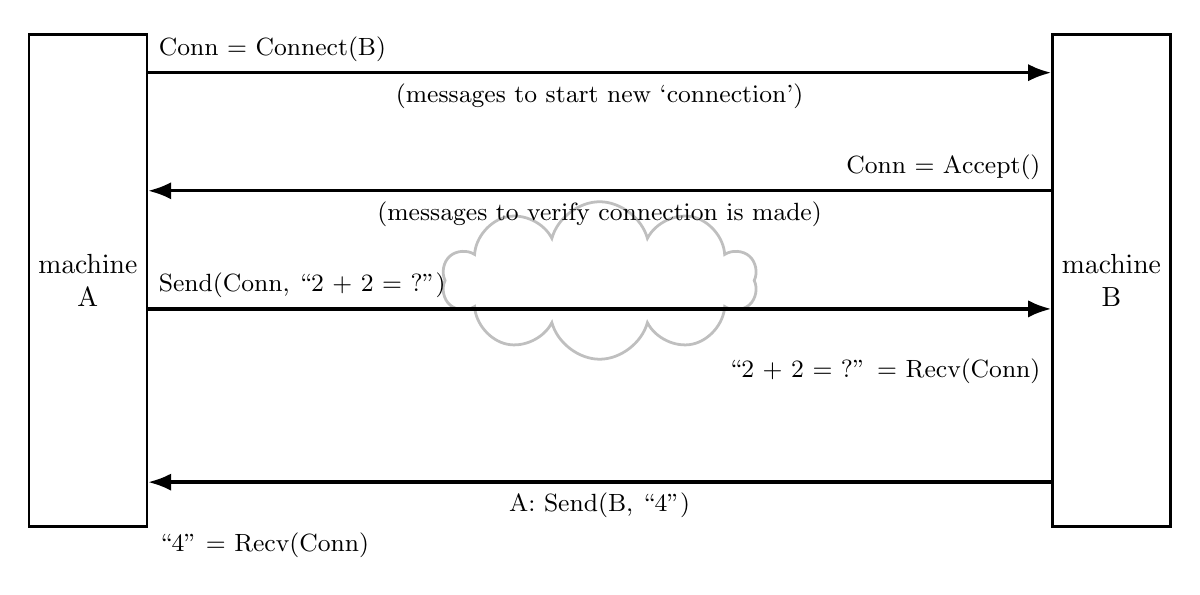
\begin{tikzpicture}
    \tikzset{
        >=Latex,
        comp box/.style={draw, thick, align=center, minimum width=1.5cm,minimum height=6.25cm},
        explain box/.style={draw=red,very thick, align=left},
        msg/.style={font=\small},
        cmd/.style={font=\small},
    }
        \node[comp box] (machine A) at (-6.5, 0) {machine \\ A};
        \node[draw,cloud,line width=1pt,minimum width=4cm,minimum height=2cm,aspect=3,opacity=0.25] (network) at (0,0) {~~};
        \node[comp box] (machine B) at (6.5, 0) {machine \\ B};
        \draw[very thick,->] ([yshift=-.5cm]machine A.north east) -- ([yshift=-.5cm]machine B.north west) 
            node[midway,below,msg] {(messages to start new `connection')}
            node[pos=0.0,above right,cmd] {Conn = Connect(B)};
        \draw[very thick,<-] ([yshift=-2cm]machine A.north east) -- ([yshift=-2cm]machine B.north west) 
            node[midway,below,msg] {(messages to verify connection is made)}
            node[pos=1.0,above left,cmd] {Conn = Accept()};
        \draw[very thick,->] ([yshift=-3.5cm]machine A.north east) -- ([yshift=-3.5cm]machine B.north west) 
            %node[midway,below,msg] {B: Send(A, ``2 + 2 = ?'')}
            node[pos=0.0,above right,cmd] {Send(Conn, ``2 + 2 = ?'')}
            node[pos=1.0,below left,cmd,yshift=-.5cm] {``2 + 2 = ?'' = Recv(Conn)};
        \draw[very thick,<-] ([yshift=-5.7cm]machine A.north east) -- ([yshift=-5.7cm]machine B.north west) 
            node[midway,below,msg] {A: Send(B, ``4'')}
            %node[pos=1.0,above left,cmd] {Send(Conn, ``4'')}
            node[pos=0.0,below right,cmd,yshift=-.5cm] {``4'' = Recv(Conn)};
    \end{tikzpicture}
\end{frame}



\section{layers preview}
\begin{frame}<1>[fragile,label=layerOverview]{networking layers}
\begin{tabular}{|l|l|p{6cm}|} \hline
application           & HTTP, SSH, SMTP, \ldots & {application-defined meanings}                                     \\ \hline
\myemph<6>{transport} & TCP, UDP, \ldots        & {reach correct program,\linebreak \myemph<2>{reliability/streams}} \\ \hline
\myemph<5>{network}   & IPv4, IPv6              & {reach correct machine}\linebreak(across networks)                 \\ \hline
\myemph<4>{link}      & Ethernet, Wi-Fi, \ldots & {coordinate shared wire/radio}                                     \\ \hline
physical              & Ethernet, Wi-Fi, \ldots & encode bits for wire/radio                                         \\ \hline
\end{tabular}
\end{frame}

\begin{frame}<1>[fragile,label=layerMsgNames]{layers terminology}
\begin{tabular}{|l|p{6cm}|l|} \hline
application & {application-defined meanings} & ~\\ \hline
transport & {reach correct program,\linebreak reliablity/streams} & segments/datagrams \\ \hline
network & {reach correct machine}\linebreak(across networks) & packets \\ \hline
link & {coordinate shared wire/radio} & frames \\ \hline
physical & encode bits for wire/radio & ~ \\ \hline
\end{tabular}
\end{frame}


\section{handling network failures}
\againframe<2>{layerOverview}

\begin{frame}<1>[label=netFailTypes]{network limitations/failures}
    \begin{itemize}
    \item \myemph<2>{messages lost}
    \item \myemph<3>{messages limited in size}
    \item \myemph<4>{messages delayed/reordered}
    \item \myemph<5>{messages corrupted}
    \end{itemize}
\end{frame}



\subsection{acknowledgments}
\againframe<2>{netFailTypes}
\usetikzlibrary{arrows.meta,shapes.misc,decorations.pathreplacing}

\begin{frame}{dealing with network message lost}
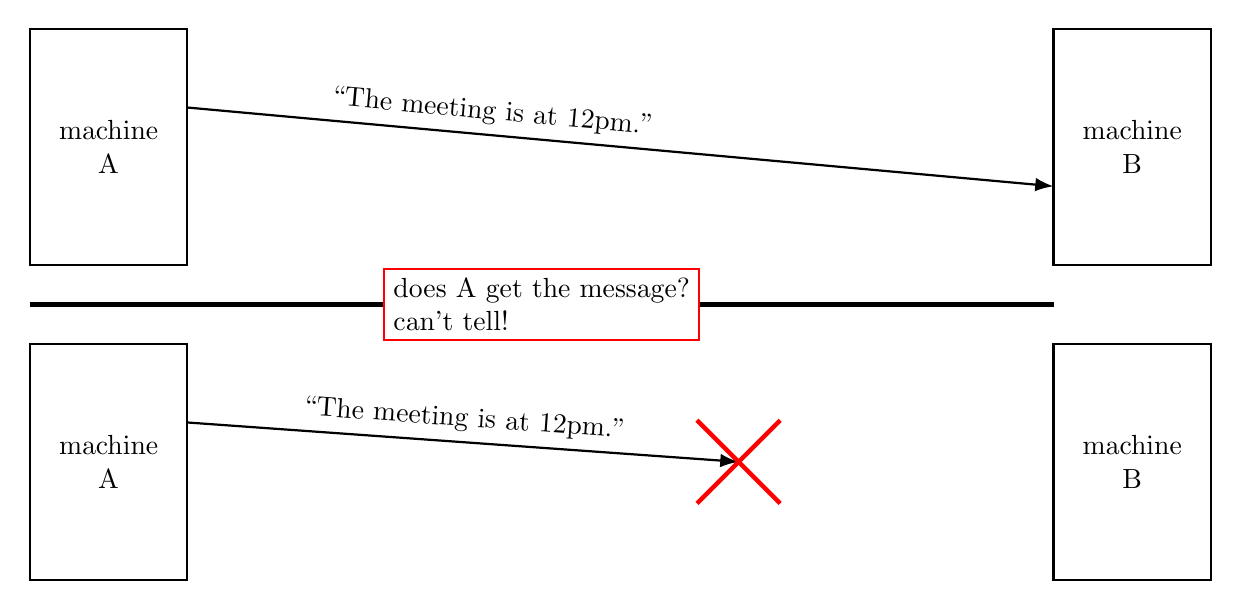
\begin{tikzpicture}
\tikzset{
    box/.style={draw,thick,minimum width=2cm},
    message/.style={draw,thick,-Latex},
    failure/.style={draw,ultra thick,red,cross out,minimum width=1cm,minimum height=1cm},
}
\begin{scope}
\draw[box] (0, 0) rectangle ++(2, -3) 
    node[midway,align=center] {machine\\ A};
\draw[box] (13, 0) rectangle ++(2, -3) 
    node[midway,align=center] {machine\\B};
\draw[message] (2, -1) -- (13, -2) node[pos=0.35, above, sloped] {``The meeting is at 12pm.''};
\end{scope}
\draw[ultra thick] (0, -3.5) -- ++ (13,0);
\begin{scope}[yshift=-4cm]
\draw[box] (0, 0) rectangle ++(2, -3) 
    node[midway,align=center] {machine\\A};
\draw[box] (13, 0) rectangle ++(2, -3) 
    node[midway,align=center] {machine\\B};
\draw[message] (2, -1) -- (9, -1.5) 
    node[pos=0.5,above,sloped] {``The meeting is at 12pm.''}
    node[failure] {};
\end{scope}
\node[draw=red,thick,fill=white,align=left] at (6.5, -3.5) {
    does A get the message? \\
    can't tell!
};
\end{tikzpicture}
\end{frame}

\begin{frame}{handling lost message: acknowledgements}
\begin{tikzpicture}
\tikzset{
    box/.style={thick},
    message/.style={draw,thick,-Latex},
    failure/.style={draw,ultra thick,red,cross out,minimum width=1cm,minimum height=1cm},
}
\begin{scope}
\draw[box] (0, 0) rectangle ++(2, -8) 
    node[midway,align=center] {machine\\A};
\draw[box] (13, 0) rectangle ++(2, -8) 
    node[midway,align=center] {machine\\B};
\draw[message] (2, -0.5) -- (13, -1) node[pos=0.35, above, sloped] {``The meeting is at 12pm.''};
\draw[message] (13, -1.5) -- (2, -2) node[pos=0.25, sloped,below] {Got it!};
\end{scope}
\end{tikzpicture}
\end{frame}

\begin{frame}{handling lost message}
\begin{tikzpicture}
\tikzset{
    box/.style={thick},
    message/.style={draw,thick,-Latex},
    failure/.style={draw,ultra thick,red,cross out,minimum width=1cm,minimum height=1cm},
}
\draw[box] (0, 0) rectangle ++(2, -8) 
    node[midway,align=center] {machine\\A};
\draw[box] (13, 0) rectangle ++(2, -8) 
    node[midway,align=center] {machine\\B};
%\draw[message] (2, -0.5) -- (13, -1) node[pos=0.35, above, sloped] {``The meeting is at 12pm.''};
\draw[message] (2, -0.5) -- (9, -1) 
    node[pos=0.5,above,sloped] {``The meeting is at 12pm.''}
    node[failure] {};
\begin{visibleenv}<2->
\draw[decorate,decoration={brace}] (2.1, -1) -- (2.1, -3) 
    node[midway,right,align=left] {
        ``timeout'' \\
        A doesn't get reply \\
        after waiting too long
    };
\end{visibleenv}
\begin{visibleenv}<3->
\draw[message] (2, -4) -- (13, -5) node[pos=0.35, above, sloped] {``The meeting is at 12pm.''};
\draw[message] (13, -5.5) -- (2, -6) node[pos=0.5, sloped,below] {Got it!};
\end{visibleenv}
\end{tikzpicture}
\end{frame}

\begin{frame}{lost acknowledgements}
\begin{tikzpicture}
\tikzset{
    box/.style={thick},
    message/.style={draw,thick,-Latex},
    failure/.style={draw,ultra thick,red,cross out,minimum width=1cm,minimum height=1cm},
}
\draw[box] (0, 0) rectangle ++(2, -8) 
    node[midway,align=center] {machine\\A};
\draw[box] (13, 0) rectangle ++(2, -8) 
    node[midway,align=center] {machine\\B};
\draw[message] (2, -0.5) -- (13, -1) node[pos=0.35, above, sloped] {``The meeting is at 12pm.''};
\draw[message] (13, -1.5) -- (6.5, -1.75) node[pos=0.5, sloped,below] {Got it!}
    node[failure] {};
\begin{visibleenv}<3->
\draw[message] (2, -3.5) -- (13, -4) node[pos=0.35, above, sloped] {``The meeting is at 12pm.''};
\draw[message] (13, -4.5) -- (2, -5) node[pos=0.5, sloped,below] {Got it!};
\end{visibleenv}
\begin{visibleenv}<2>
\node[draw=red,thick,fill=white,align=left] at (6.5, -6.5) {
    A's going to need to resend this message! \\
    Can't tell it really was received!
};
\end{visibleenv}
\begin{visibleenv}<3>
\node[draw=red,thick,fill=white,align=left] at (6.5, -6.5) {
    B needs to handle receiving message twice! \\
    Sockets: you only get a copy of the data once.
};
\end{visibleenv}
\end{tikzpicture}
\end{frame}


\begin{frame}{delayed acknowledgements}
\begin{tikzpicture}
\tikzset{
    box/.style={thick},
    message/.style={draw,thick,-Latex},
    failure/.style={draw,ultra thick,red,cross out,minimum width=1cm,minimum height=1cm},
}
\draw[box] (0, 0) rectangle ++(2, -8) 
    node[midway,align=center] {machine\\A};
\draw[box] (13, 0) rectangle ++(2, -8) 
    node[midway,align=center] {machine\\B};
\draw[message] (2, -0.5) -- (13, -1) node[pos=0.35, above, sloped] {``The meeting is at 12pm.''};
\draw[message] (13, -1.5) -- (2, -5) node[pos=0.25, sloped,below] {Got it!};
\draw[decorate,decoration={brace}] (2.1, -1) -- (2.1, -3) 
    node[midway,right,align=left] {
        ``timeout''
    };
\begin{visibleenv}<3->
\draw[message] (2, -3.5) -- (13, -4) node[pos=0.35, above, sloped] {``The meeting is at 12pm.''};
\draw[message] (13, -4.5) -- (2, -6) node[pos=0.5, sloped,below] {Got it!};
\end{visibleenv}
\begin{visibleenv}<3>
\node[draw=red,thick,fill=white,align=left] at (8, -6.5) {
    B can't tell that first acknowledgment wasn't lost
};
\end{visibleenv}
\end{tikzpicture}
\end{frame}

\subsubsection{exercise: lost acks}
\begin{frame}{exercise: lost acknowledgement}
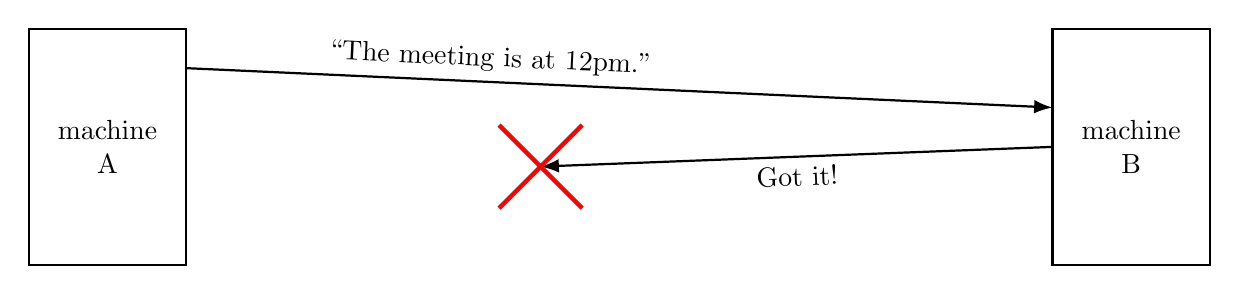
\begin{tikzpicture}
\tikzset{
    box/.style={thick},
    message/.style={draw,thick,-Latex},
    failure/.style={draw,ultra thick,red,cross out,minimum width=1cm,minimum height=1cm},
}
\draw[box] (0, 0) rectangle ++(2, -3) 
    node[midway,align=center] {machine\\A};
\draw[box] (13, 0) rectangle ++(2, -3) 
    node[midway,align=center] {machine\\B};
\draw[message] (2, -0.5) -- (13, -1) node[pos=0.35, above, sloped] {``The meeting is at 12pm.''};
\draw[message] (13, -1.5) -- (6.5, -1.75) node[pos=0.5, sloped,below] {Got it!}
    node[failure] {};
\end{tikzpicture}
exercise: how to fix this?
\begin{tabular}{ll}
A. & machine A needs to send ``Got `got it!' '' \\
B. & machine B should resend ``Got it!'' on its own \\
C. & machine A should resend the original message on its own \\
D. & none of these \\
\end{tabular}
\end{frame}

\begin{frame}<0>[label=lostAckExExplain]{answers}
\begin{itemize}
\item send ``Got `got it!' ''?
    \begin{itemize}
    \item same problem: Now send `Got Got Got it'?
    \end{itemize}
\item resend ``Got it!'' own its own?
    \begin{itemize}
    \item how many times? --- B doesn't have that info
    \end{itemize}
\item resend original message?
    \begin{itemize}
    \item yes!
    \item as far as machine A can see, \textit{exact same situation} as losing original message
    \end{itemize}
\end{itemize}
\end{frame}

\iftoggle{heldback}{}{
    \againframe<1>{lostAckExExplain}
}


\subsubsection{solution: lost acks}
\iftoggle{heldback}{}{

\begin{frame}{lost acknowledgements}
\begin{tikzpicture}
\tikzset{
    box/.style={thick},
    message/.style={draw,thick,-Latex},
    failure/.style={draw,ultra thick,red,cross out,minimum width=1cm,minimum height=1cm},
}
\draw[box] (0, 0) rectangle ++(2, -8) 
    node[midway,align=center] {machine\\A};
\draw[box] (13, 0) rectangle ++(2, -8) 
    node[midway,align=center] {machine\\B};
\draw[message] (2, -0.5) -- (13, -1) node[pos=0.35, above, sloped] {``The meeting is at 12pm.''};
\draw[message] (13, -1.5) -- (6.5, -1.75) node[pos=0.5, sloped,below] {Got it!}
    node[failure] {};
\begin{visibleenv}<3->
\draw[message] (2, -3.5) -- (13, -4) node[pos=0.35, above, sloped] {``The meeting is at 12pm.''};
\draw[message] (13, -4.5) -- (2, -5) node[pos=0.5, sloped,below] {Got it!};
\end{visibleenv}
\begin{visibleenv}<2>
\node[draw=red,thick,fill=white,align=left] at (6.5, -6.5) {
    A's going to need to resend this message! \\
    Can't tell it really was received!
};
\end{visibleenv}
\begin{visibleenv}<3>
\node[draw=red,thick,fill=white,align=left] at (6.5, -6.5) {
    B needs to handle receiving message twice! \\
    Sockets: you only get a copy of the data once.
};
\end{visibleenv}
\end{tikzpicture}
\end{frame}
}
\subsubsection{delayed acks}
\againframe<3>{netFailTypes}

\begin{frame}{delayed message}
\begin{tikzpicture}
\tikzset{
    box/.style={thick},
    message/.style={draw,thick,-Latex},
    failure/.style={draw,ultra thick,red,cross out,minimum width=1cm,minimum height=1cm},
}
\draw[box] (0, 0) rectangle ++(2, -8) 
    node[midway,align=center] {machine\\A};
\draw[box] (13, 0) rectangle ++(2, -8) 
    node[midway,align=center] {machine\\B};
\draw[message] (2, -0.5) -- (13, -4.5) node[pos=0.35, above, sloped] {``The meeting is at 12pm.''};
\draw[message] (13, -4.5) -- (2, -5) node[pos=0.25, sloped,below] {Got it!};
\draw[decorate,decoration={brace}] (2.1, -1) -- (2.1, -3) 
    node[midway,right,align=left] {
        ``timeout''
    };
\begin{visibleenv}<3->
\draw[message] (2, -3.5) -- (13, -5) node[pos=0.35, above, sloped] {``The meeting is at 12pm.''};
\draw[message] (13, -5.5) -- (2, -6) node[pos=0.5, sloped,below] {Got it!};
\end{visibleenv}
\begin{visibleenv}<3>
\node[draw=red,thick,fill=white,align=left] at (8, -7) {
    B resends, can't tell message is just slow
};
\end{visibleenv}
\end{tikzpicture}
\end{frame}


\begin{frame}{delayed acknowledgements}
\begin{tikzpicture}
\tikzset{
    box/.style={thick},
    message/.style={draw,thick,-Latex},
    failure/.style={draw,ultra thick,red,cross out,minimum width=1cm,minimum height=1cm},
}
\draw[box] (0, 0) rectangle ++(2, -8) 
    node[midway,align=center] {machine\\A};
\draw[box] (13, 0) rectangle ++(2, -8) 
    node[midway,align=center] {machine\\B};
\draw[message] (2, -0.5) -- (13, -1) node[pos=0.35, above, sloped] {``The meeting is at 12pm.''};
\draw[message] (13, -1.5) -- (2, -5) node[pos=0.25, sloped,below] {Got it!};
\draw[decorate,decoration={brace}] (2.1, -1) -- (2.1, -3) 
    node[midway,right,align=left] {
        ``timeout''
    };
\begin{visibleenv}<3->
\draw[message] (2, -3.5) -- (13, -4) node[pos=0.35, above, sloped] {``The meeting is at 12pm.''};
\draw[message] (13, -4.5) -- (2, -6) node[pos=0.5, sloped,below] {Got it!};
\end{visibleenv}
\begin{visibleenv}<3>
\node[draw=red,thick,fill=white,align=left] at (8, -6.5) {
    B can't tell that first acknowledgment wasn't lost
};
\end{visibleenv}
\end{tikzpicture}
\end{frame}



\subsection{splitting into multiple}
\againframe<4>{netFailTypes}
\usetikzlibrary{arrows.meta,decorations.pathreplacing,shapes.misc}

\begin{frame}{splitting messages: try 1}
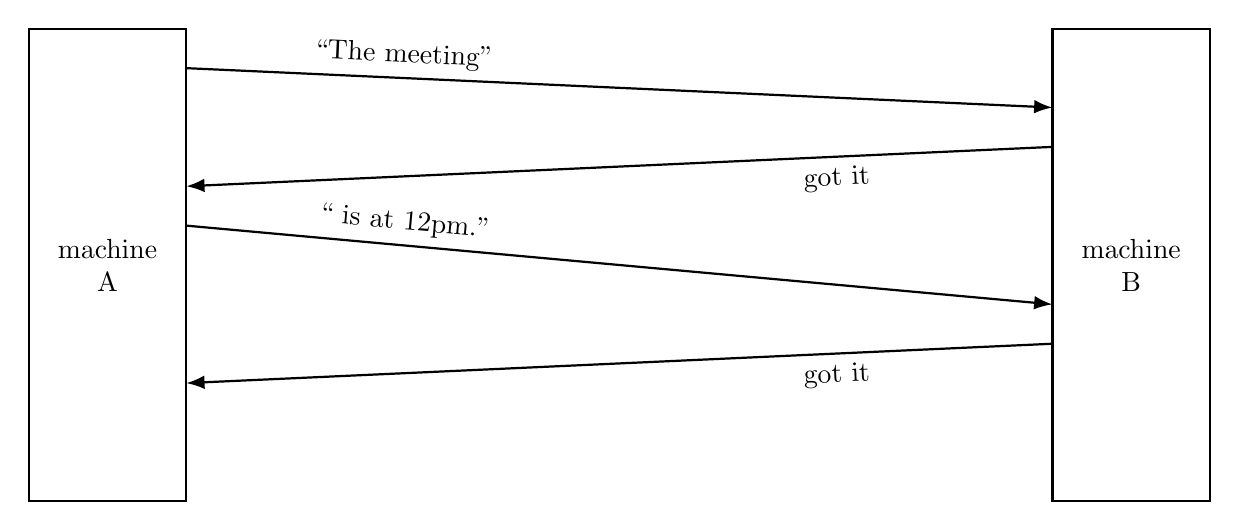
\begin{tikzpicture}
\tikzset{
    box/.style={thick},
    message/.style={draw,thick,-Latex},
    failure/.style={draw,ultra thick,red,cross out,minimum width=1cm,minimum height=1cm},
}
\begin{scope}
\draw[box] (0, 0) rectangle ++(2, -6) 
    node[midway,align=center] {machine\\A};
\draw[box] (13, 0) rectangle ++(2, -6) 
    node[midway,align=center] {machine\\B};
\draw[message] (2, -0.5) -- (13, -1) node[pos=0.25, above, sloped] {``The meeting''};
\draw[message] (13, -1.5) -- (2, -2) node[pos=0.25, sloped,below] {got it};
\draw[message] (2, -2.5) -- (13, -3.5) node[pos=0.25, above, sloped] {`` is at 12pm.''};
\draw[message] (13, -4) -- (2, -4.5) node[pos=0.25, sloped,below] {got it};
\end{scope}
\end{tikzpicture}
reconstructed message: \\
The meeting is at 12pm.
\end{frame}


\begin{frame}{splitting messages: try 1 --- problem}
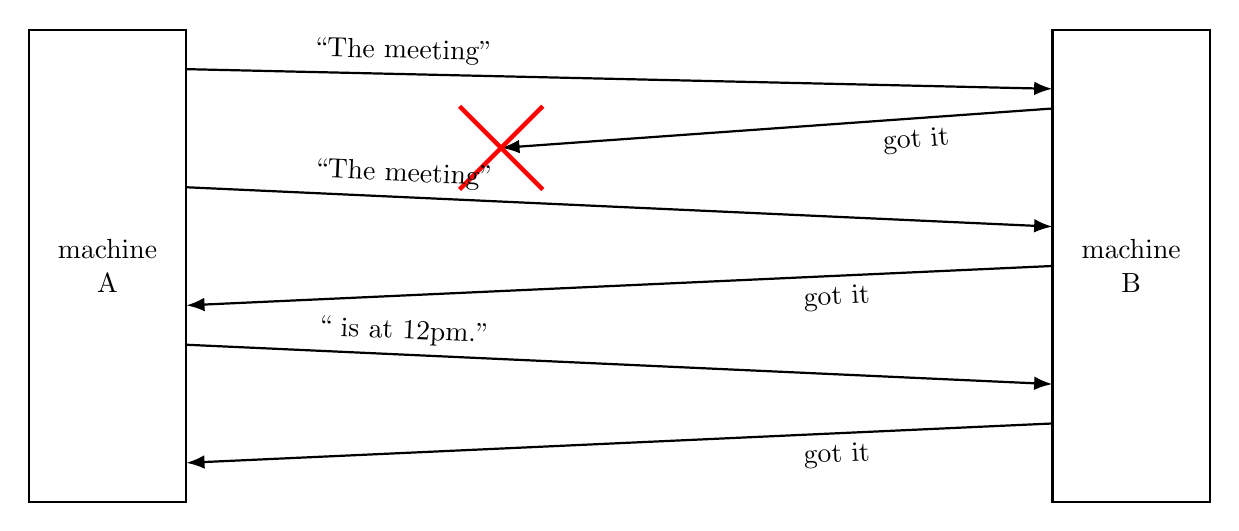
\begin{tikzpicture}
\tikzset{
    box/.style={thick},
    message/.style={draw,thick,-Latex},
    failure/.style={draw,ultra thick,red,cross out,minimum width=1cm,minimum height=1cm},
}
\begin{scope}
\draw[box] (0, 0) rectangle ++(2, -6) 
    node[midway,align=center] {machine\\A};
\draw[box] (13, 0) rectangle ++(2, -6) 
    node[midway,align=center] {machine\\B};
\draw[message] (2, -0.5) -- (13, -0.75) node[pos=0.25, above, sloped] {``The meeting''};
\draw[message] (13, -1) -- (6, -1.5) node[pos=0.25, sloped,below] {got it} node[failure] {};
\draw[message] (2, -2) -- (13, -2.5) node[pos=0.25, above, sloped] {``The meeting''};
\draw[message] (13, -3) -- (2, -3.5) node[pos=0.25, sloped,below] {got it};
\draw[message] (2, -4) -- (13, -4.5) node[pos=0.25, above, sloped] {`` is at 12pm.''};
\draw[message] (13, -5) -- (2, -5.5) node[pos=0.25, sloped,below] {got it};
\end{scope}
\end{tikzpicture}
reconstructed message: \\
The meetingThe meeting is at 12pm.
\end{frame}

\begin{frame}{splitting messages: try 2}
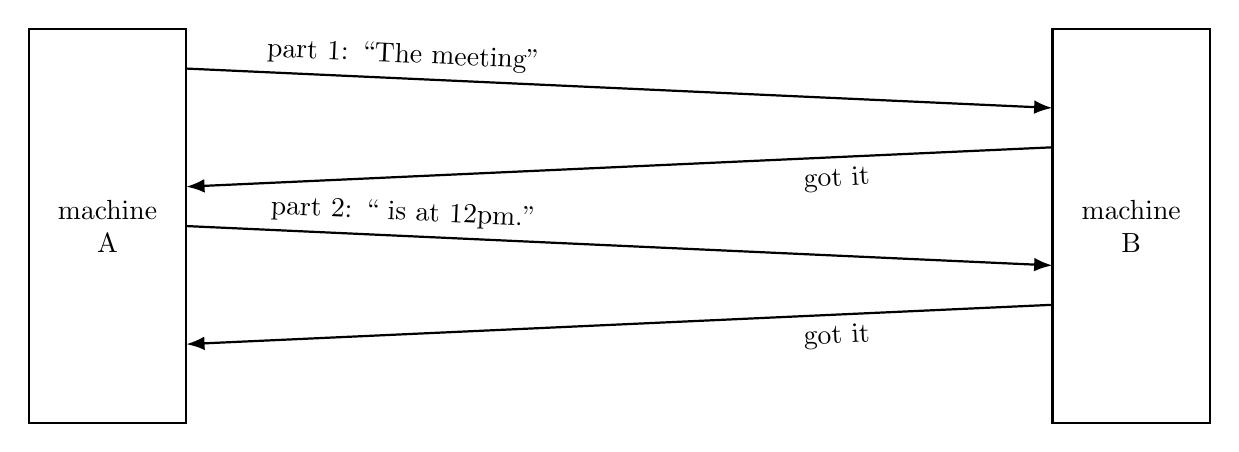
\begin{tikzpicture}
\tikzset{
    box/.style={thick},
    message/.style={draw,thick,-Latex},
    failure/.style={draw,ultra thick,red,cross out,minimum width=1cm,minimum height=1cm},
}
\begin{scope}
\draw[box] (0, 0) rectangle ++(2, -5) 
    node[midway,align=center] {machine\\A};
\draw[box] (13, 0) rectangle ++(2, -5) 
    node[midway,align=center] {machine\\B};
\draw[message] (2, -0.5) -- (13, -1) node[pos=0.25, above, sloped] {part 1: ``The meeting''};
\draw[message] (13, -1.5) -- (2, -2) node[pos=0.25, sloped,below] {got it};
\draw[message] (2, -2.5) -- (13, -3) node[pos=0.25, above, sloped] {part 2: `` is at 12pm.''};
\draw[message] (13, -3.5) -- (2, -4) node[pos=0.25, sloped,below] {got it};
\end{scope}
\end{tikzpicture}
reconstructed message: \\
The meeting is at 12pm.
\end{frame}

\begin{frame}{splitting messages: try 2 --- missed ack}
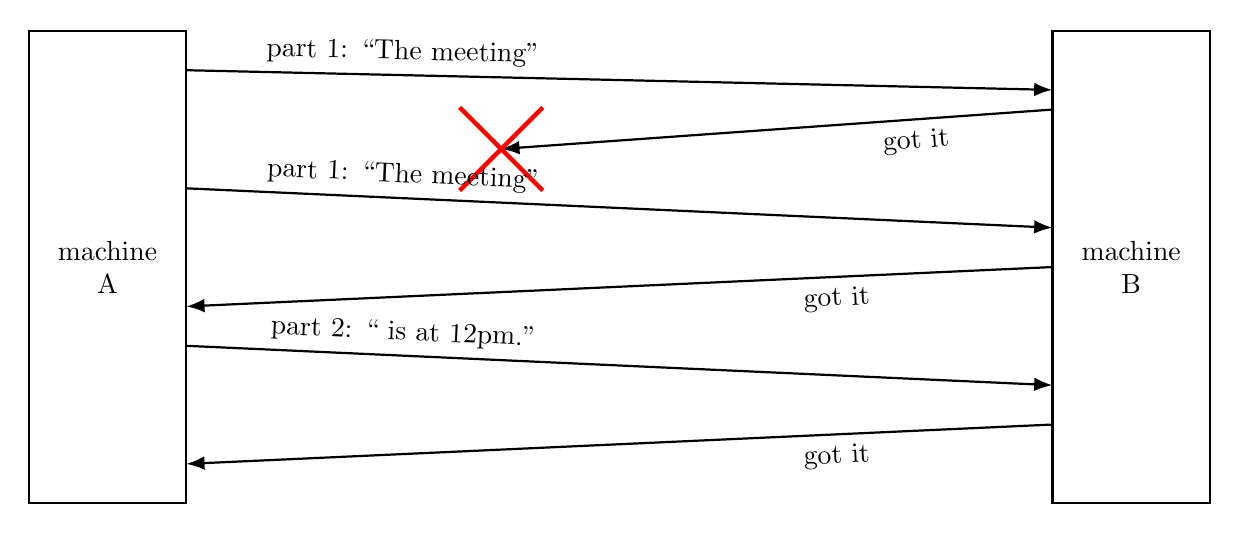
\begin{tikzpicture}
\tikzset{
    box/.style={thick},
    message/.style={draw,thick,-Latex},
    failure/.style={draw,ultra thick,red,cross out,minimum width=1cm,minimum height=1cm},
}
\begin{scope}
\draw[box] (0, 0) rectangle ++(2, -6) 
    node[midway,align=center] {machine\\A};
\draw[box] (13, 0) rectangle ++(2, -6) 
    node[midway,align=center] {machine\\B};
\draw[message] (2, -0.5) -- (13, -0.75) node[pos=0.25, above, sloped] {part 1: ``The meeting''};
\draw[message] (13, -1) -- (6, -1.5) node[pos=0.25, sloped,below] {got it} node[failure] {};
\draw[message] (2, -2) -- (13, -2.5) node[pos=0.25, above, sloped] {part 1: ``The meeting''};
\draw[message] (13, -3) -- (2, -3.5) node[pos=0.25, sloped,below] {got it};
\draw[message] (2, -4) -- (13, -4.5) node[pos=0.25, above, sloped] {part 2: `` is at 12pm.''};
\draw[message] (13, -5) -- (2, -5.5) node[pos=0.25, sloped,below] {got it};
\end{scope}
\end{tikzpicture}
reconstructed message: \\
The meeting is at 12pm.
\end{frame}

\begin{frame}{splitting messages: try 2 --- problem}
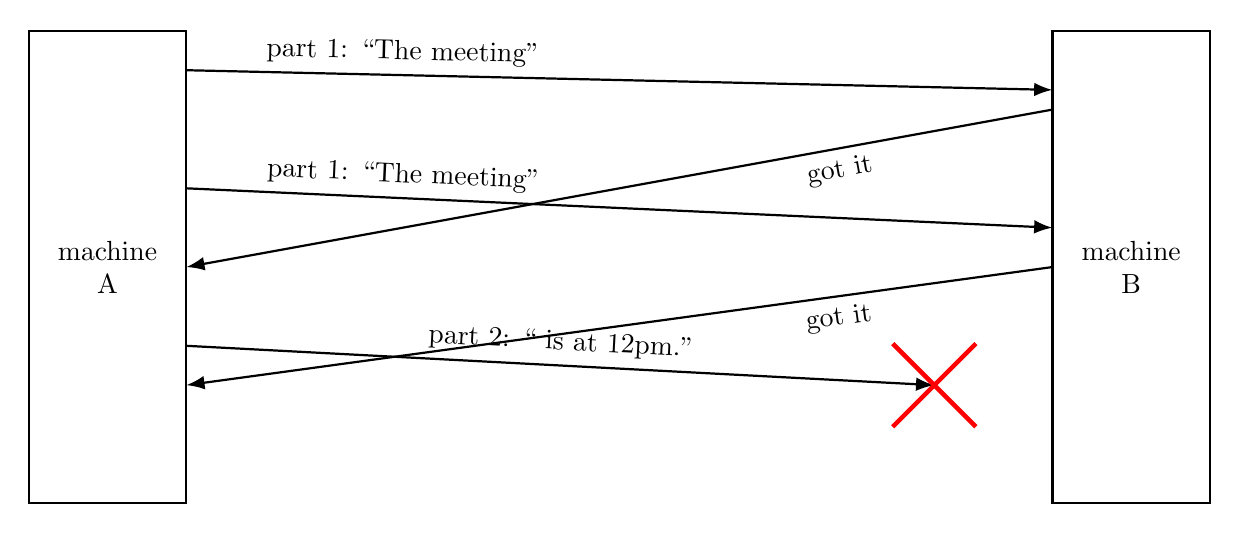
\begin{tikzpicture}
\tikzset{
    box/.style={thick},
    message/.style={draw,thick,-Latex},
    failure/.style={draw,ultra thick,red,cross out,minimum width=1cm,minimum height=1cm},
}
\begin{scope}
\draw[box] (0, 0) rectangle ++(2, -6) 
    node[midway,align=center] {machine\\A};
\draw[box] (13, 0) rectangle ++(2, -6) 
    node[midway,align=center] {machine\\B};
\draw[message] (2, -0.5) -- (13, -0.75) node[pos=0.25, above, sloped] {part 1: ``The meeting''};
\draw[message] (13, -1) -- (2, -3) node[pos=0.25, sloped,below] {got it};
\draw[message] (2, -2) -- (13, -2.5) node[pos=0.25, above, sloped] {part 1: ``The meeting''};
\draw[message] (13, -3) -- (2, -4.5) node[pos=0.25, sloped,below] {got it};
\draw[message] (2, -4) -- (11.5, -4.5) node[pos=0.5, above, sloped] {part 2: `` is at 12pm.''}
    node[failure] {};
\end{scope}
\end{tikzpicture}
A thinks: part 1 + part 2 acknowleged!
\end{frame}

\begin{frame}{splitting messages: version 3}
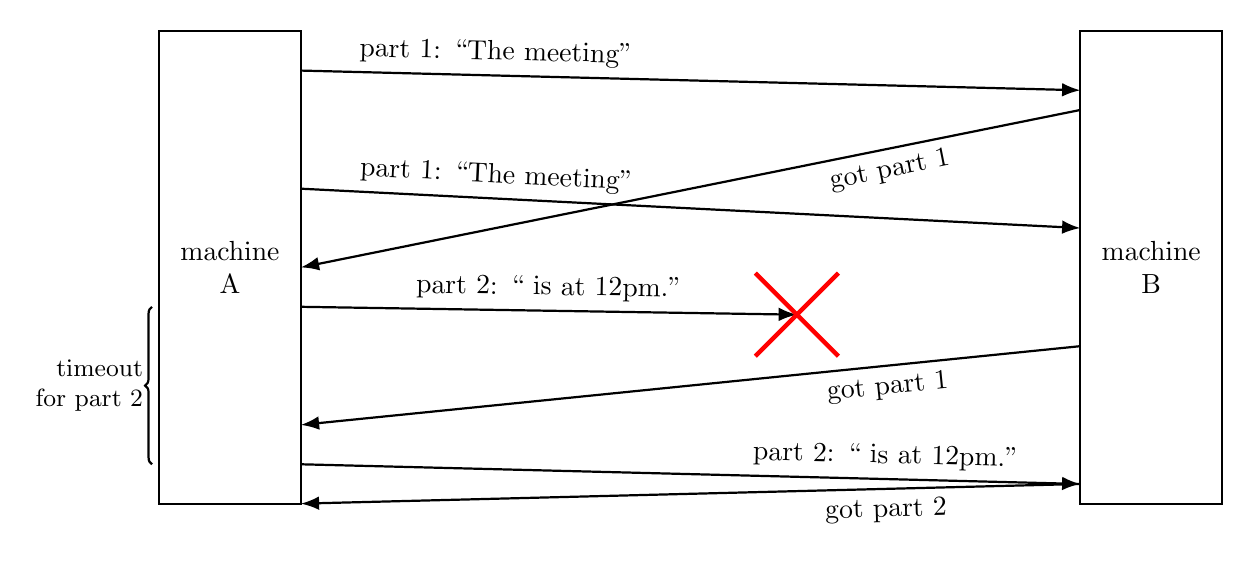
\begin{tikzpicture}
\tikzset{
    box/.style={thick},
    message/.style={draw,thick,-Latex},
    failure/.style={draw,ultra thick,red,cross out,minimum width=1cm,minimum height=1cm},
}
\begin{scope}[xshift=1cm,x=0.9cm]
\draw[box] (0, 0) rectangle ++(2, -6) 
    node[midway,align=center] {machine\\A};
\draw[box] (13, 0) rectangle ++(2, -6) 
    node[midway,align=center] {machine\\B};
\draw[message] (2, -0.5) -- (13, -0.75) node[pos=0.25, above, sloped] {part 1: ``The meeting''};
\draw[message] (13, -1) -- (2, -3) node[pos=0.25, sloped,below] {got \myemph{part 1}};
\draw[message] (2, -2) -- (13, -2.5) node[pos=0.25, above, sloped] {part 1: ``The meeting''};
\draw[message] (13, -4) -- (2, -5) node[pos=0.25, sloped,below] {got \myemph{part 1}};
\draw[message] (2, -3.5) -- (9, -3.6) node[pos=0.5, above, sloped] {part 2: `` is at 12pm.''}
    node[failure] {};
\draw[thick,decorate,decoration={brace,mirror}] (-0.1, -3.5) -- (-0.1, -5.5) node[inner sep=1mm,font=\small,align=right,midway,left] {timeout\\\myemph{for part 2}};
\draw[message] (2, -5.5) -- (13, -5.75) node[pos=0.75, above, sloped] {part 2: `` is at 12pm.''};
\draw[message] (13, -5.75) -- (2, -6) node[pos=0.25, below, sloped] {got \myemph{part 2}};
\end{scope}
\end{tikzpicture}
\end{frame}


    % FIXME: exercise
        % acknowledge only last
        % partial acknowledgments

\subsection{checksums}
\againframe<5>{netFailTypes}
\begin{frame}{message corrupted}
\begin{itemize}
\item instead of sending ``message''
\vspace{.5cm}
\item say Hash(``message'') = 0xABCDEF12
\item then send ``0xABCDEF12,message''
\vspace{.5cm}
\item when receiving, recompute hash
\item pretend message lost if does not match
\end{itemize}
\end{frame}

\begin{frame}{``checksum''}
\begin{itemize}
\item these hashes commonly called ``checksums''
\item in UDP/TCP, hash function: treat bytes of messages as array of integers; then add integers together
\end{itemize}
\end{frame}

    % FIXME: exercise: 

\subsection{aside: going faster}
\begin{frame}{going faster}
    \begin{itemize}
    \item so far: send one message, wait for acknowledgment
    \vspace{.5cm}
    \item very slow!
    \item instead, can send a bunch of parts and get them acknowledged together
    % \item need to do \textit{congestion control} to avoid overloading network
    \end{itemize}
\end{frame}

\usetikzlibrary{arrows.meta,decorations.pathreplacing,shapes.misc}

\begin{frame}{transmission window (ex: size 4)}
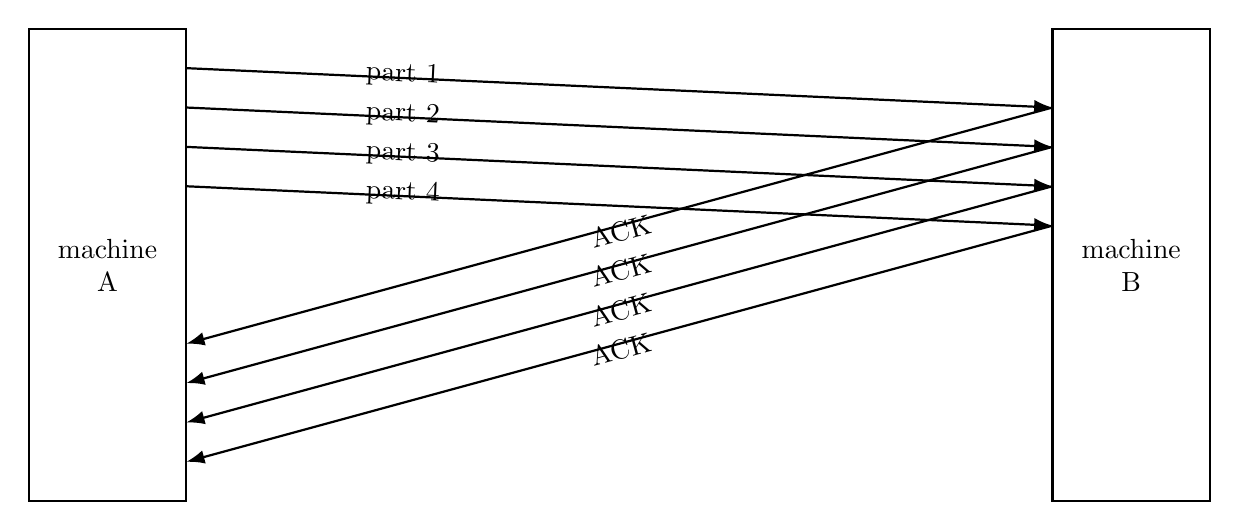
\begin{tikzpicture}
\tikzset{
    box/.style={thick},
    message/.style={draw,thick,-Latex},
    failure/.style={draw,ultra thick,red,cross out,minimum width=1cm,minimum height=1cm},
}
\begin{scope}
\draw[box] (0, 0) rectangle ++(2, -6)
    node[midway,align=center] {machine\\A};
\draw[box] (13, 0) rectangle ++(2, -6)
    node[midway,align=center] {machine\\B};
\draw[message] (2, -0.5) -- (13, -1.0) node[pos=0.25, above=-7pt, sloped] {part 1};
\draw[message] (2, -1.0) -- (13, -1.5) node[pos=0.25, above=-7pt, sloped] {part 2};
\draw[message] (2, -1.5) -- (13, -2.0) node[pos=0.25, above=-7pt, sloped] {part 3};
\draw[message] (2, -2.0) -- (13, -2.5) node[pos=0.25, above=-7pt, sloped] {part 4};
\draw[message] (13, -1.0) -- (2, -4.0) node[pos=0.5, sloped, below=-5pt] {ACK};
\draw[message] (13, -1.5) -- (2, -4.5) node[pos=0.5, sloped, below=-5pt] {ACK};
\draw[message] (13, -2.0) -- (2, -5.0) node[pos=0.5, sloped, below=-5pt] {ACK};
\draw[message] (13, -2.5) -- (2, -5.5) node[pos=0.5, sloped, below=-5pt] {ACK};
\end{scope}
\end{tikzpicture}
Send a \textit{window} of parts speculatively, then wait for ACKs.
\end{frame}


\section{layers, revisited}
\againframe<3>{layerOverview}

\begin{frame}{more than four layers?}
    \begin{itemize}
    \item sometimes more layers above `application'
    \item e.g. HTTPS:
        \begin{itemize}
        \item HTTP (app layer) on TLS (another app layer) on TCP (network) on \ldots
        \end{itemize}
    \item e.g. DNS over HTTPS:
        \begin{itemize}
        \item DNS (app layer) on HTTP on on TLS on TCP on \ldots
        \end{itemize}
    \item e.g. SFTP:
        \begin{itemize}
        \item SFTP (app layer??) on SSH (another app layer) on TCP on \ldots
        \end{itemize}
    \item e.g. HTTP over OpenVPN:
        \begin{itemize}
        \item HTTP on TCP on IP on OpenVPN on UDP on different IP on \ldots
        \end{itemize}
    \end{itemize}
\end{frame}


\section{addresses versus names}
\usetikzlibrary{arrows.meta,calc,positioning,shapes.callouts,shapes.symbols}

\begin{frame}{names and addresses}
\small
\begin{tabular}{l|l}
\textbf{name} & \textbf{address} \\\hline
\large\myemph{logical identifier} & \large\myemph{location/how to locate} \\
~ & ~ \\
variable \texttt{counter} & memory address \texttt{0x7FFF9430} \\ 
~ & ~ \\
DNS name \texttt{www.virginia.edu} & IPv4 address \texttt{128.143.22.36} \\
DNS name \texttt{mail.google.com} & IPv4 address \texttt{216.58.217.69} \\
DNS name \texttt{mail.google.com} & IPv6 address \fontsize{10}{11}\selectfont\texttt{2607:f8b0:4004:80b::2005} \\
    DNS name \fontsize{10}{11}\selectfont\texttt{reiss-t3620.cs.virginia.edu} & IPv4 address \texttt{128.143.67.91} \\
    DNS name \fontsize{10}{11}\selectfont\texttt{reiss-t3620.cs.virginia.edu} & MAC address \texttt{18:66:da:2e:7f:da} \\
~ & ~ \\
service name \texttt{https} & port number \texttt{443} \\
service name \texttt{ssh} & port number \texttt{22} \\
\end{tabular}
\end{frame}



\section{a frame example}
\againframe<4>{layerOverview}
\usetikzlibrary{decorations.pathreplacing,fit,matrix}
\begin{frame}{an Ethernet frame}
\begin{tikzpicture}
\tikzset{
    small label/.style={font=\small},
    box/.style={thick},
}
\matrix[tight matrix no line,
    nodes={font=\tt\small\strut,text width=0.7cm},
] {
|[alias=destMacStart]| 4c \& cc \& 6a \& ba \& 1c \& |[alias=destMacEnd]| b9 \& 
|[alias=sourceMacStart]| d8 \& 07 \& b6 \& d9 \& ae \& |[alias=sourceMacEnd]| 50 \&
|[alias=etherTypeStart]| 08 \& |[alias=etherTypeEnd]| 00 \\[1cm]
|[alias=ipTypeHLen,alias=ipHeadStart]| \alt<2->{\setlength{\fboxsep}{0pt}\colorbox{orange!20}{4}}{4}5 \& 
|[alias=ipDiffServ]| 00 \& 
|[alias=ipLenStart]| 00 \& |[alias=ipLenEnd]| 60\&
|[alias=ipIdStart]| db \& |[alias=ipIdEnd]| 89 \&
|[alias=ipFlagsAndFragStart]| 40 \& |[alias=ipFlagsAndFragEnd]| 00 \& 
|[alias=ipTTL]| f2 \& 
|[alias=ipProto]| 06 \& 
|[alias=ipChkSumSt]| cf \& |[alias=ipChkSumEnd]| cd \&
|[alias=ipSrcStart]| 34 \& 60 \& e6 \& |[alias=ipSrcEnd,alias=ipFirstLine]| a2 \\[1cm]
|[alias=ipDstStart]| c0 \& a8 \& 01 \& |[alias=ipDstEnd]| 95 \&
|[alias=tcpHeadStart,alias=srcPortStart]| 01 \& |[alias=srcPortEnd]| bb \& |[alias=dstPortStart]| aa \& |[alias=dstPortEnd]| c4 \& |[alias=seqNumStart]| 40 \& 2b \& d6 \& |[alias=seqNumEnd]| 46 \& 
    |[alias=ackNumStart]| 7c \& 9d \& 15 \& |[alias=tcpHeadFirstLine,alias=ackNumEnd]| e4 \\[.7cm] 
|[alias=tcpSecondLine,alias=tcpFlagsStart]| 80 \& |[alias=tcpFlagsEnd]| 18 \& |[alias=tcpWinStart]| 40 \& |[alias=tcpWinEnd]| 02 \& 
|[alias=checkSumStart]| 65 \& |[alias=checkSumEnd]| fe \& |[alias=urgentStart]| 00 \& |[alias=urgentEnd]| 00 \&
|[alias=tcpOptStart]| 01 \& 01 \& 08 \& 0a \& 03 \& 83 \& 98 \& 62 \\[.7cm]
19 \& 70 \& 27 \& |[alias=tcpOptEnd]| 9e \& |[alias=tcpDataStart]| 17 \& 03 \& 03 \& 00 \& 27 \& 00 \& 00 \& 00 \& 00 \& 00 \& 00 \& |[alias=tcpDataFirstLine]| 00 \\
|[alias=tcpDataSecondLine]| c8 \& b9 \& ab \& 81 \& 50 \& e0 \& ef \& 1a \& d8 \& 97 \& 73 \& 76 \& 9a \& ee \& 33 \& d4 \\
 9a \& cb \& 17 \& 29 \& f0 \& fa \& 1c \& 13 \& 4c \& b0 \& 07 \& ef \& 92 \& 8b \& 0a \& |[alias=tcpEnd]| a9 \\
};
\begin{pgfonlayer}{bg}
    \tikzset{
        every label/.style={font=\small\bfseries,align=center},
        every node/.style={label distance=-0.5mm},
    }
    \node[fill=blue!20,inner sep=0mm, fit=(destMacStart) (destMacEnd),label={[fill=blue!20]north:destination\\MAC address}] {};
    \node[fill=violet!20,inner sep=0mm, fit=(sourceMacStart) (sourceMacEnd),label={[fill=violet!20]north:source\\MAC address}] {};
    \node[fill=yellow!30,inner sep=0mm, fit=(etherTypeStart) (etherTypeEnd),label={[fill=yellow!30]north:frame\\type}] {};
    \begin{visibleenv}<1>
    \node[fill=red!20,very thick,inner sep=0mm,fit=(ipHeadStart) (tcpEnd),label={[fill=red!20]north:frame's data}] {};
    \end{visibleenv}
    \begin{visibleenv}<2->
    \draw[very thick,decorate,decoration={brace}] ([yshift=.7cm,xshift=1.9cm]ipFirstLine.north east) -- ([xshift=1.9cm]tcpEnd.south east) node[midway,right,font=\small,align=left] {IP\\packet};
    \node[font=\small\bfseries,align=center,anchor=south,fill=orange!20,overlay] at ([yshift=-2mm,xshift=.25cm]ipTypeHLen.north west) {vers.};
    %\node[font=\small\bfseries,align=center,anchor=south west,fill=violet!20] at ([yshift=-2mm,xshift=-.5cm] ipTypeHLen.north east) {h. len.};
    \node[fill=green!20,inner sep=0mm, fit=(ipLenStart) (ipLenEnd),label={[fill=green!20]north:length}] {};
    \node[fill=yellow!20,inner sep=0mm, fit=(ipProto),label={[fill=yellow!20]north:protocol}] {};
    \node[fill=blue!20,inner sep=0mm, fit=(ipDstStart) (ipDstEnd),label={[fill=blue!20]north:destination\\IPv4 address}] {};
    \node[fill=violet!20,inner sep=0mm, fit=(ipSrcStart) (ipSrcEnd),label={[fill=violet!20]north:source\\IPv4 address}] {};
    \end{visibleenv}
    \begin{visibleenv}<2>
    \path[fill=red!20] (tcpHeadStart.north west) -- (tcpHeadFirstLine.north east) -- (tcpEnd.south east) -| (tcpSecondLine.north west) -| cycle;
    \node[anchor=south,fill=red!20,font=\small\bfseries] at ([xshift=2cm,yshift=-2mm]tcpHeadStart.north) {packet's data};
    \end{visibleenv}
    \begin{visibleenv}<3->
    \draw[very thick,decorate,decoration={brace}] ([xshift=.2cm]tcpHeadFirstLine.north east) -- ([xshift=.2cm]tcpEnd.south east) node[midway,right,font=\small,align=left] {TCP\\segment};
    \node[fill=blue!20,inner sep=0mm, fit=(dstPortStart) (dstPortEnd),label={[fill=blue!20]north:dest.\\port}] {};
    \node[fill=violet!20,inner sep=0mm, fit=(srcPortStart) (srcPortEnd),label={[fill=violet!20]north:source\\port}] {};
    \node[fill=orange!20,inner sep=0mm, fit=(seqNumStart) (seqNumEnd),label={[fill=orange!20]north:sequence num.}] {};
    \node[fill=orange!20,inner sep=0mm, fit=(tcpFlagsStart) (tcpFlagsEnd),label={[fill=orange!20]north:flags}] {};
    \path[fill=red!20] (tcpDataStart.north west) -- (tcpDataFirstLine.north east) -- (tcpEnd.south east) -| (tcpDataSecondLine.north west) -| cycle;
    \node[anchor=south,fill=red!20,font=\small\bfseries] at ([xshift=2cm,yshift=-2mm]tcpDataStart.north) {segment's data};
    \path[draw,dotted,very thick] ([xshift=0mm]tcpHeadStart.north west) |- ([yshift=7mm]tcpSecondLine.north west) -- (tcpSecondLine.west |- tcpEnd.south east);
    \end{visibleenv}
\end{pgfonlayer}
\end{tikzpicture}
\end{frame}


\section{ethernet / 802.11 / \ldots}
\begin{frame}{the link layer}
\begin{itemize}
\item Ethernet, Wi-Fi, Bluetooth, DOCSIS (cable modems), \ldots
\vspace{.5cm}
\item allows send/recv messages to machines on \myemph<2>{``same'' network segment}
    \begin{itemize}
    \item typically: wireless range+channel or connected to a single switch/router
    \item could be larger (if \textit{bridging} multiple network segments)
    \item could be smaller (switch/router uses ``virtual LANs'')
    \end{itemize}
\item typically: source+destination specified with MAC addresses
    \begin{itemize}
    \item MAC = media access control
    \item usually manufacturer assigned / hard-coded into device
    \item unique address per port/wifi transmitter/etc.
    \end{itemize}
\item can specify destination of ``anyone'' (called \textit{broadcast})
\item messages usually called ``frames''
\end{itemize}
\end{frame}

\begin{frame}{link layer jobs}
    \begin{itemize}
    \item divide raw bits into messages
    \item identify who message is for on shared radio/wire
    \item handle if two+ machines use radio/wire at same time
    \item drop/resend messages if corruption detected
        \begin{itemize}
        \item resending more common in radio schemes (wifi, etc.)
        \end{itemize}
    \end{itemize}
\end{frame}


\subsection{exercise: why resend?}
\begin{frame}{link layer reliablity?}
    \begin{itemize}
    \item Ethernet + Wifi have checksums
    \vspace{.5cm}
    \item Q1: Why doesn't this give us uncorrupted messages?
        \begin{itemize}
        \item Why do we still have checksums at the higher layers?
        \end{itemize}
    \item Q2: What's a benefit of doing this if we're also doing it in the higher layer?
    \end{itemize}
\end{frame}


\section{IP}

% FIXME: example sending message multiple hop
\againframe<5>{layerOverview}
\usetikzlibrary{calc,positioning,shapes.callouts}

\begin{frame}{the network layer}
\begin{itemize}
\item the Internet Protocool (IP) version 4 or version 6
    \begin{itemize}
    \item there are also others, but quite uncommon today
    \end{itemize}
\item allows send messages to/recv messages from other networks
    \begin{itemize}
    \item ``internetwork''
    \end{itemize}
\item messages usually called ``packets''
\end{itemize}
\end{frame}

\begin{frame}[fragile]{network layer quality of service}
if packet \ldots \\
\small
\begin{tabular}{l|p{12cm}}
event & on IPv4/v6 \\\hline
collides with another & out of scope --- handled by link layer \\
\myemph<2>{not received}\tikzmark{not recv} & lost silently \\
header corrupted & usually discarded silently \\
data corrupted & received corrupted \\
too long & dropped with notice or ``fragmented'' + recombined \\
reordered (v. other messages) & received out of order \\
destination unknown & usually dropped with notice \\
too much being sent & discard excess \\
\end{tabular}
\begin{tikzpicture}[overlay,remember picture]
\begin{visibleenv}<2>
\node[align=left,my callout=not recv,anchor=north west] at ([xshift=0cm,yshift=-3cm]pic cs:not recv) {
    includes dropped by link layer \\
    (e.g. if detected corrupted there)
};
\end{visibleenv}
\end{tikzpicture}
\end{frame}


\subsection{IPv4 addresses}
\begin{frame}{IPv4 addresses}
    \begin{itemize}
    \item 32-bit numbers
    \item typically written like 128.143.67.11
        \begin{itemize}
        \item four 8-bit decimal values separated by dots
        \item first part is most significant
        \item same as $128\cdot 256^3+143\cdot 256^2 + 67\cdot256 + 11 = 2\,156\,782\,459$
        \end{itemize}
    \vspace{.5cm}
    \item organizations get blocks of IPs
    \begin{itemize}
        \item e.g. UVa has 128.143.0.0--128.143.255.255
        \item e.g. Google has 216.58.192.0--216.58.223.255 and 74.125.0.0--74.125.255.255 and 35.192.0.0--35.207.255.255
    \end{itemize}
    \item some IPs reserved for non-Internet use (127.*, 10.*, 192.168.*)
    \end{itemize}
\end{frame}



\subsection{IPv6 addresses}
\begin{frame}{IPv6 addresses}
    \begin{itemize}
    \item IPv6 like IPv4, but with 128-bit numbers
    \item written in hex, 16-bit parts, seperated by colons (\texttt{:})
    \item strings of 0s represented by double-colons (\texttt{::})
    \item typically given to users in blocks of $2^{80}$ or $2^{64}$ addresses
        \begin{itemize}
        \item no need for address translation?
        \end{itemize}
    \vspace{.5cm}
    \item \fontsize{10}{11}\selectfont\texttt{2607:f8b0:400d:c00::6a} = \\
          \texttt{2607:f8b0:400d:0c00:0000:0000:0000:006a}
          \begin{itemize}
          \item \texttt{2607f8b0400d0c0000000000000006a}$_\text{SIXTEEN}$
          \end{itemize}
    \end{itemize}
\end{frame}

\begin{frame}{selected special IPv6 addresses}
    \begin{itemize}
    \item \texttt{::1} = localhost
    \item anything starting with \texttt{fe80} = link-local addresses
        \begin{itemize}
        \item never forwarded by routers
        \end{itemize}
    \end{itemize}
\end{frame}



\subsection{routing idea}

\begin{frame}{IPv4 addresses and routing tables}
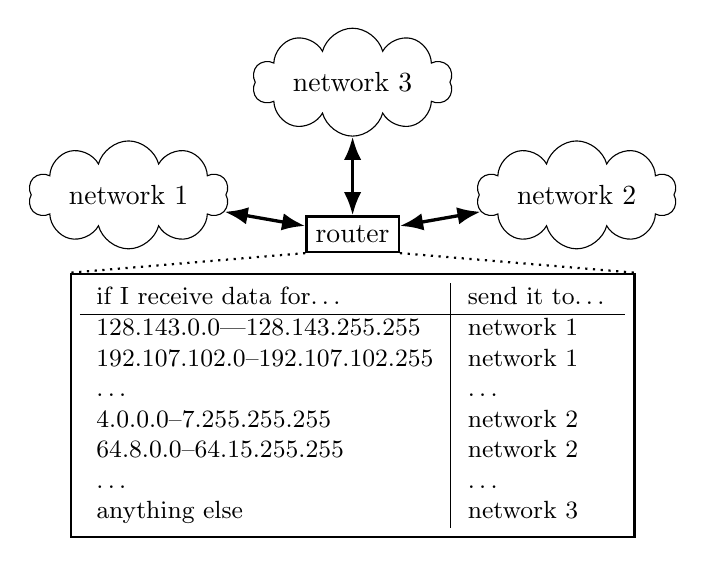
\begin{tikzpicture}
\tikzset{>=Latex},
\node[draw,thick] (router) {router};
\node[aspect=3,draw,cloud,anchor=east,minimum width=2.5cm] (network 1) at ([xshift=-1cm,yshift=.5cm] router.west) {
    network 1
};
\node[aspect=3,draw,cloud,anchor=west,minimum width=2.5cm] (network 2) at ([xshift=1cm,yshift=.5cm] router.east) {
    network 2
};
\node[aspect=3,draw,cloud,anchor=south,minimum width=2.5cm] (network 3) at ([yshift=1cm] router.north) {
    network 3
};
\foreach \x in {1,2,3} { \draw[<->,very thick] (router) -- (network \x); }
\node[anchor=north,font=\small,draw,thick] (table) at ([yshift=-.25cm]router.south) {
\begin{tabular}{l|l}
if I receive data for\ldots & send it to\ldots \\ \hline
128.143.0.0---128.143.255.255 & network 1 \\
192.107.102.0--192.107.102.255 & network 1 \\
\ldots & \ldots \\
4.0.0.0--7.255.255.255 & network 2 \\
64.8.0.0--64.15.255.255 & network 2 \\
\ldots & \ldots \\
anything else & network 3 \\
\end{tabular}
};
\draw[thick,dotted] (router.south west) -- (table.north west);
\draw[thick,dotted] (router.south east) -- (table.north east);
\end{tikzpicture}
\end{frame}




\subsection{special addresses}
\begin{frame}{selected special IPv4 addresses}
\begin{itemize}
\item 127.0.0.0 --- 127.255.255.255 --- localhost
    \begin{itemize}
    \item AKA loopback
    \item the machine we're on
    \item typically only 127.0.0.1 is used
    \end{itemize}
\item 192.168.0.0--192.168.255.255 and \\ 10.0.0.0--10.255.255.255 and \\ 172.16.0.0--172.31.255.255 
    \begin{itemize}
    \item ``private'' IP addresses
    \item not used on the Internet
    \item commonly connected to Internet with \myemph{network address translation}
    \item also 100.64.0.0--100.127.255.255 (but with restrictions)
    \end{itemize}
\item 169.254.0.0-169.254.255.255
    \begin{itemize}
    \item link-local addresses --- `never' forwarded by routers
    \end{itemize}
\end{itemize}
\end{frame}



\section{TCP/UDP}
\againframe<6>{layerOverview}

\subsection{port numbers}
\begin{frame}{port numbers}
    \begin{itemize}
    \item we run multiple programs on a machine
        \begin{itemize}
        \item IP addresses identifying machine --- not enough
        \end{itemize}
    \item<2-> so, add 16-bit \textit{port numbers}
        \begin{itemize}
        \item<2-> think: multiple PO boxes at address
        \end{itemize}
    \vspace{.5cm}
    \item<3-> 0--49151: typically assigned for particular services
        \begin{itemize}
        \item 80 = http, 443 = https, 22 = ssh, \ldots
        \end{itemize}
    \item<3-> 49152--65535: allocated on demand
        \begin{itemize}
        \item default ``return address'' for client connecting to server
        \end{itemize}
    \end{itemize}
\end{frame}



\subsection{UDP v TCP}
\begin{frame}[fragile]{UDP v TCP}
    \begin{itemize}
    \item UDP: messages sent to program, but no reliablity/streams
        \begin{itemize}
        \item \texttt{SOCK\_DGRAM} with socket() instead of \texttt{SOCK\_STREAM}
        \item can sendto()/recvfrom() multiple other programs with one socket
            \begin{itemize}
            \item (but don't have to)
            \end{itemize}
        \item send messages which are limited in size, unreliable
        \end{itemize}
    \item TCP: stream to other program
        \begin{itemize}
        \item need to bind() + listen() + accept() or connect() to setup connection
        \item one socket per connection
        \item read/write bytes --- divided into messages automatically
        \item reliable --- acknowledgments/resending handled for you
        \end{itemize}
    \end{itemize}
\end{frame}


\subsection{UDP sockets}
\begin{frame}[fragile]{UDP sockets on IPv4}
\begin{lstlisting}[language=C++,style=smaller]
int fd = socket(AF_INET, SOCK_DGRAM, 0);
struct sockaddr_in my_addr= ...;
bind(fd, &my_addr, sizeof(my_addr))
...
struct sockaddr_in to_addr = ...;
sendto(fd, data, data_size, 0 /* flags */,
    &to_addr, sizeof(to_addr));
struct sockaddr_in from_addr = ...;
recvfrom(fd, &buffer[0], buffer_size, 0,
    &from_addr, sizeof(from_addr));
...
/* or connect() to set default sendto address
\end{lstlisting}
\end{frame}


\subsection{OS tracking connections}
\begin{frame}{connections in TCP/IP}
    \begin{itemize}
    \item connection identified by \textit{5-tuple}
        \begin{itemize}
        \item used by OS to lookup ``where is the socket?''
        \end{itemize}
    \item \small(protocol=TCP/UDP, local IP addr., local port, remote IP addr., remote port)
    \vspace{.5cm}
    \item local IP address, port number can be set with \texttt{bind()} function
        \begin{itemize}
        \item \textit{typically} always done for servers, not done for clients
        \item system will choose default if you don't
        \end{itemize}
    \end{itemize}
\end{frame}

\begin{frame}[fragile,label=laptopNetstat]{connections on my desktop}
\begin{lstlisting}[language={},basicstyle=\fontsize{9.5}{10.5}\selectfont]
cr4bd@reiss-t3620>/u/cr4bd
$ netstat --inet --inet6 --numeric
Active Internet connections (w/o servers)
Proto Recv-Q Send-Q Local Address           Foreign Address         State      
tcp        0      0 128.143.67.91:49202     128.143.63.34:22        ESTABLISHED
tcp        0      0 128.143.67.91:803       128.143.67.236:2049     ESTABLISHED
tcp        0      0 128.143.67.91:50292     128.143.67.226:22       TIME_WAIT  
tcp        0      0 128.143.67.91:54722     128.143.67.236:2049     TIME_WAIT  
tcp        0      0 128.143.67.91:52002     128.143.67.236:111      TIME_WAIT  
tcp        0      0 128.143.67.91:732       128.143.67.236:63439    TIME_WAIT  
tcp        0      0 128.143.67.91:40664     128.143.67.236:2049     TIME_WAIT  
tcp        0      0 128.143.67.91:54098     128.143.67.236:111      TIME_WAIT  
tcp        0      0 128.143.67.91:49302     128.143.67.236:63439    TIME_WAIT  
tcp        0      0 128.143.67.91:50236     128.143.67.236:111      TIME_WAIT  
tcp        0      0 128.143.67.91:22        172.27.98.20:49566      ESTABLISHED
tcp        0      0 128.143.67.91:51000     128.143.67.236:111      TIME_WAIT  
tcp        0      0 127.0.0.1:50438         127.0.0.1:631           ESTABLISHED
tcp        0      0 127.0.0.1:631           127.0.0.1:50438         ESTABLISHED
\end{lstlisting}
\end{frame}

\begin{frame}{non-connection sockets}
\begin{itemize}
\item TCP servers waiting for connections + \\
UDP sockets with no particular remote host
\item Linux: OS keeps 5-tuple with ``wildcard'' remote address
\end{itemize}
\end{frame}

\begin{frame}[fragile,label=laptopNetstat]{``listening'' sockets on my desktop}
\begin{lstlisting}[language={},basicstyle=\fontsize{9.5}{10.5}\selectfont]
cr4bd@reiss-t3620>/u/cr4bd
$ netstat --inet --inet6 --numeric --listen
Active Internet connections (only servers)
Proto Recv-Q Send-Q Local Address           Foreign Address         State      
tcp        0      0 127.0.0.1:38537         0.0.0.0:*               LISTEN     
tcp        0      0 127.0.0.1:36777         0.0.0.0:*               LISTEN     
tcp        0      0 0.0.0.0:41099           0.0.0.0:*               LISTEN     
tcp        0      0 0.0.0.0:45291           0.0.0.0:*               LISTEN     
tcp        0      0 127.0.0.1:51949         0.0.0.0:*               LISTEN     
tcp        0      0 127.0.0.1:41071         0.0.0.0:*               LISTEN     
tcp        0      0 0.0.0.0:111             0.0.0.0:*               LISTEN     
tcp        0      0 127.0.0.1:32881         0.0.0.0:*               LISTEN     
tcp        0      0 127.0.0.1:38673         0.0.0.0:*               LISTEN     
....
tcp6       0      0 :::42689                :::*                    LISTEN
udp        0      0 128.143.67.91:60001     0.0.0.0:*
udp        0      0 128.143.67.91:60002     0.0.0.0:*
...
udp6       0      0 :::59938                :::* 
\end{lstlisting}
\end{frame}


\subsection{aside: TCP state machine}
\begin{frame}{TCP state machine}
\begin{itemize}
\item TIME\_WAIT, ESTABLISHED, \ldots?
\vspace{.5cm}
\item OS tracks ``state'' of TCP connection
    \begin{itemize}
    \item am I just starting the connection?
    \item is other end ready to get data?
    \item am I trying to close the connection?
    \item do I need to resend something?
    \end{itemize}
\item standardized set of state names
\end{itemize}
\end{frame}


\begin{frame}{TIME\_WAIT}
\begin{itemize}
\item remember delayed messages?
\vspace{.5cm}
\item problem for TCP ports
\item if I reuse port number, I can get message from old connection
\item solution: TIME\_WAIT to make sure connection really done
    \begin{itemize}
    \item done after sending last message in connection
    \end{itemize}
\end{itemize}
\end{frame}
 % FIXME: diagram

\section{DNS}
\againframe<2>{nameAndAddr}
\usetikzlibrary{arrows.meta,positioning,shapes.callouts}
\begin{frame}[fragile,label=dnsDD]{DNS: distributed database}
\begin{tikzpicture}
    \tikzset{
        >=Latex,
        comp box/.style={draw, thick, align=center, minimum width=1.5cm,minimum height=1.5cm},
        explain box/.style={draw=red,very thick, align=left},
        msg/.style={font=\small},
        cmd/.style={font=\small},
        my callout2/.style={draw,fill=blue!10!white,rectangle callout,callout absolute pointer=(#1),below right=5pt of {#1}}
    }
    \node[comp box] (my machine) at (0, 0) { my \\ machine };
    \node[comp box] (isp) at (6, 0) { ISP's \\ DNS server };
    \begin{visibleenv}<1>
        \node[my callout2=isp.south,fill=red!10,align=center,font=\small,anchor=north] at ([xshift=-2cm,yshift=-2cm]isp.south) {
            address sent to my machine \\
            when it connected to network
        };
    \end{visibleenv}
    \begin{visibleenv}<3->
    \node[comp box] (root) at (11, 2) { root \\ DNS server };
    \end{visibleenv}
    \begin{visibleenv}<4->
    \node[comp box] (edu) at (11, 0) { .edu \\ DNS server };
    \node[comp box] (virginia) at (11, -2) { virginia.edu \\ DNS server };
    \node[comp box] (cs) at (11, -4) { {\small cs.virginia.edu} \\ DNS server };
    \end{visibleenv}
    \begin{visibleenv}<2->
    \draw[very thick,<->] (my machine) -- (isp)
        coordinate[midway] (midpt);
    \node[my callout2=midpt,anchor=south,font=\fontsize{9}{10}\selectfont,align=left] at ([yshift=1cm]midpt) {
        address for \\ www.cs.virginia.edu?
    };
    \end{visibleenv}
    \begin{visibleenv}<5->
    \node[my callout2=midpt,anchor=north,font=\fontsize{9}{10}\selectfont,align=left] at ([yshift=-1cm]midpt) {
        www.cs.virginia.edu = \\
        128.143.67.11
    };
    \end{visibleenv}
    \foreach \n/\when in {root/3,edu/4,virginia/4,cs/4} {
        \draw[very thick,<->,alt=<\when->{}{invisible}] (isp) -- (\n.west) coordinate[midway] (midpt \n);
    }
    \begin{visibleenv}<3->
        \node[my callout2=midpt root,anchor=south,font=\fontsize{9}{10}\selectfont,align=left,
              alt=<5>{fill=red!10}] at ([yshift=1cm]midpt root) {
            www.cs.virginia.edu? \\
            try .edu server at \ldots
        };
        \begin{visibleenv}<5>
            \draw[very thick,dotted,red,<->] (isp) -- (root.west);
            \node[draw=red,very thick,fill=white,align=left,anchor=north,font=\small] at ([yshift=-3cm]midpt root) {
                .edu server doesn't change much \\
                optimization: \textit{cache} its address \\
                ~ \\
                check for updated version once in a while
            };
        \end{visibleenv}
    \end{visibleenv}
\end{tikzpicture}
\end{frame}


% FIXME: DNS dig example
\subsection{DNS: dig +trace}

\begin{frame}[fragile]{querying the root}
\begin{Verbatim}[fontsize=\scriptsize]
$ dig @a.root-servers.net www.cs.virginia.edu
...
edu.			172800	IN	NS	b.edu-servers.net.
edu.			172800	IN	NS	f.edu-servers.net.
edu.			172800	IN	NS	i.edu-servers.net.
edu.			172800	IN	NS	a.edu-servers.net.
...
b.edu-servers.net.	172800	IN	A	192.33.14.30
b.edu-servers.net.	172800	IN	AAAA	2001:503:231d::2:30
f.edu-servers.net.	172800	IN	A	192.35.51.30
f.edu-servers.net.	172800	IN	AAAA	2001:503:d414::30
...
\end{Verbatim}
\end{frame}

\begin{frame}[fragile]{querying the edu}
\begin{Verbatim}[fontsize=\scriptsize]
$ dig @b.edu-servers.net www.cs.virginia.edu
...
;; AUTHORITY SECTION:
virginia.edu.		172800	IN	NS	nom.virginia.edu.
virginia.edu.		172800	IN	NS	uvaarpa.virginia.edu.
virginia.edu.		172800	IN	NS	eip-01-aws.net.virginia.edu.

;; ADDITIONAL SECTION:
nom.virginia.edu.	172800	IN	A	128.143.107.101
uvaarpa.virginia.edu.	172800	IN	A	128.143.107.117
eip-01-aws.net.virginia.edu. 172800 IN	A	44.234.207.10
\end{Verbatim}
\end{frame}
\begin{frame}[fragile]{querying virginia.edu}
\begin{Verbatim}[fontsize=\scriptsize]
$ dig @nom.virginia.edu www.cs.virginia.edu
...
;; AUTHORITY SECTION:
cs.virginia.edu.	3600	IN	NS	coresrv01.cs.virginia.edu.

;; ADDITIONAL SECTION:
coresrv01.cs.virginia.edu. 3600	IN	A	128.143.67.11
\end{Verbatim}
\end{frame}

\begin{frame}[fragile]{querying cs.virginia.edu}
\begin{Verbatim}[fontsize=\scriptsize]
$ dig @coresrv01.cs.virginia.edu
...
;; ANSWER SECTION:
www.cs.Virginia.EDU.	172800	IN	A	128.143.67.11

;; AUTHORITY SECTION:
cs.Virginia.EDU.	172800	IN	NS	coresrv01.cs.Virginia.EDU.
...
\end{Verbatim}
\end{frame}

\begin{frame}[fragile]{querying typical ISP's resolver}
\begin{Verbatim}[fontsize=\scriptsize]
$ dig www.cs.virginia.edu
...
;; ANSWER SECTION:
www.cs.Virginia.EDU.	  7183	IN	A	128.143.67.11
..
\end{Verbatim}
\begin{itemize}
\item cached response
\item valid for 7183  more seconds
\item after that everyone needs to check again
\end{itemize}
\end{frame}


\subsection{ARP / IPv6 ND}
\againframe<3>{nameAndAddr}
\begin{frame}{two types of addresses?}
    \begin{itemize}
    \item MAC addreses: on link layer
    \item IP addresses: on network layer
    \vspace{.5cm}
    \item how do we know which MAC address to use?
    \end{itemize}
\end{frame}

\begin{frame}[fragile]{a table on my desktop}
my desktop: \\
\begin{Verbatim}[fontsize=\fontsize{9}{10}\selectfont]
$ arp -an
? (128.143.67.140) at 3c:e1:a1:18:bd:5f [ether] on enp0s31f6
? (128.143.67.236) at <incomplete> on enp0s31f6
? (128.143.67.11) at 30:e1:71:5f:39:10 [ether] on enp0s31f6
? (128.143.67.92) at <incomplete> on enp0s31f6
? (128.143.67.5) at d4:be:d9:b0:99:d1 [ether] on enp0s31f6
\end{Verbatim}
\ldots
\end{frame}

\begin{frame}{how is that table made?}
    \begin{itemize}
    \item ask machines on local network (same switch)
    \item ``Who has 128.148.67.140''
    \item the correct one replies
    \end{itemize}
\end{frame}

\begin{frame}{what about non-local machines?}
    \begin{itemize}
    \item when configuring network specify:
    \vspace{.5cm}
    \item range of addresses to expect on local network 
        \begin{itemize}
        \item 128.148.67.0-128.148.67.255 on my desktop
        \item ``netmask''
        \end{itemize}
    \item \textit{gateway} machine to send to for things outside my local network
        \begin{itemize}
        \item 128.143.67.1 on my desktop
        \item my desktop looks up the corresponding MAC address
        \end{itemize}
    \end{itemize}
\end{frame}

\begin{frame}[fragile]{routes on my desktop}
\begin{Verbatim}[fontsize=\fontsize{9}{10}\selectfont]
$ /sbin/route -n
Kernel IP routing table
Destination     Gateway         Genmask         Flags Metric Ref    Use Iface
0.0.0.0         128.143.67.1    0.0.0.0         UG    100    0        0 enp0s31f6
128.143.67.0    0.0.0.0         255.255.255.0   U     100    0        0 enp0s31f6
169.254.0.0     0.0.0.0         255.255.0.0     U     1000   0        0 enp0s31f6
\end{Verbatim}
\begin{itemize}
\item network configuration says:
\vspace{.5cm}
\item (line 2) to get to 128.143.67.0--128.143.67.255, send directly on local network
    \begin{itemize}
    \item ``genmask'' is mask (for bitwise operations) to specify how big range is
    \end{itemize}
\item (line 3) to get to 169.254.0.0--169.254.255.255, send directly on local network
\item (line 1) to get anywhere else, use ``gateway'' 128.143.67.1
\end{itemize}
\end{frame}


\subsection{URLs and URIs}
\begin{frame}{URL / URIs}
\begin{itemize}
\item Uniform Resource Locators (URL)
    \begin{itemize}
    \item tells how to find ``resource'' on network
    \end{itemize}
\item Unifrom Resources Identifiers
    \begin{itemize}
    \item superset of URLs
    \end{itemize}
\end{itemize}
\end{frame}

\begin{frame}[fragile]{URI examples}
\begin{Verbatim}[fontsize=\small]
https://kytos02.cs.virginia.edu:443/cs3130-spring2023/
                quizzes/quiz.php?qid=02#q2

https://kytos02.cs.virginia.edu/cs3130-spring2023/
                quizzes/quiz.php?qid=02

https://www.cs.virginia.edu/

sftp://cr4bd@portal.cs.virginia.edu/u/cr4bd/file.txt

tel:+1-434-982-2200
\end{Verbatim}
\end{frame}


\begin{frame}[fragile]{URI generally}
\begin{Verbatim}
scheme://authority/path?query#fragment
\end{Verbatim}
\begin{itemize}
\item scheme: --- what protocol
\item //authority/
    \begin{itemize}
    \item authoirty = user@host:port OR host:port OR user@host OR host
    \end{itemize}
\item path
    \begin{itemize}
    \item which resource
    \end{itemize}
\item ?query --- usually key/value pairs 
\item \#fragment --- place in resource
\vspace{.5cm}
\item most components (sometimes) optional
\end{itemize}
\end{frame}


% FIXME: HTTP request/response?
\section{and HTTP? (exercise)}
\begin{frame}[fragile]{URLs and HTTP (1)}
\begin{itemize}
    \item \texttt{http://www.foo.com:80/foo/bar?quux\myemph<2>{\#q1}}
    \item lookup IP address of www.foo.com
    \item connect via TCP to port 80:
\end{itemize}
\providecommand{\emphThree}[1]{\myemph<3>{#1}}
\begin{Verbatim}[commandchars=X()]
GET /foo/bar?quux HTTP/1.1
Host: XemphThree(www.foo.com:80)
\end{Verbatim}
\begin{itemize}
    \item<3-> exercise: why include the Host there?
\end{itemize}
\end{frame}



\section{DHCP and IPv6 autoconfig}

\begin{frame}{autoconfiguration}
\begin{itemize}
\item problem: how does my machine get IP address
\vspace{.5cm}
\item otherwise:
    \begin{itemize}
    \item have sysadmin type one in?
    \item just choose one?
    \item \myemph<2>{ask machine on local network to assign it}
    \end{itemize}
\vspace{.5cm}
\item<3-> often local router machine runs service to assign IP addresses
    \begin{itemize}
    \item knows what IP addresses are available
    \item sysadmin might configure in mapping from MAC addresses to IP addresses
    \end{itemize}
\end{itemize}
\end{frame}

\begin{frame}{DHCP high-level}
    \begin{itemize}
    \item protocol done over UDP
    \vspace{.5cm}
    \item but since we don't have IP address yet, use \texttt{0.0.0.0}
    \item and since we don't know server address, use \texttt{255.255.255.255}
        \begin{itemize}
        \item = ``everyone on the local network''
        \end{itemize}
    \item local server replies to request with address + \myemph<2>{time limit}
    \item later: can send messages to local server to renew/give up address
    \end{itemize}
\end{frame}

\begin{frame}{exercise: why time limit?}
    \begin{itemize}
        \item DHCP ``lease''
        \item rather than getting address forever
        \vspace{.5cm}
        \item but DHCP has way of releasing taken address
        \vspace{.5cm}
        \item why impose a time limit
    \end{itemize}
\end{frame}




\section{firewalls} % FIXME: complete
\begin{frame}{firewalls}
    \begin{itemize}
    \item don't want to expose network service to everyone?
    \item solutions:
        \begin{itemize}
        \item service picky about who it accepts connections from
        \item filters in OS on machine with services
        \item filters on router
        \end{itemize}
    \item later two called ``firewalls''
    \end{itemize}
\end{frame}

\begin{frame}{firewall rules examples?}
    \begin{itemize}
    \item ALLOW tcp port 443 (https) FROM everyone
    \item ALLOW tcp port 22 (ssh) FROM \myemph{my desktop's IP address}
    \item BLOCK tcp port 22 (ssh) FROM everyone else
    \item ALLOW from address X to address Y
    \item \ldots
    \end{itemize}
\end{frame}


% FIXME: update readings to mention IPv6 equivalent

\section{spoofing?}
\begin{frame}{spoofing}
    \begin{itemize}
    \item if I only allow connections from my desktop's IP addresses, \\
        how would you attack this?
    \vspace{.5cm}
    \item hint: how do we know what address messages come from?
    \end{itemize}
\end{frame}


\section{backup slides}

\begin{frame}{The Internet}
    \begin{itemize}
    \item Perhaps the most successful computer application ever
    \item Can you name a computer program that doesn't use the internet?
    \end{itemize}
\end{frame}

\begin{frame}{}
\begin{center}
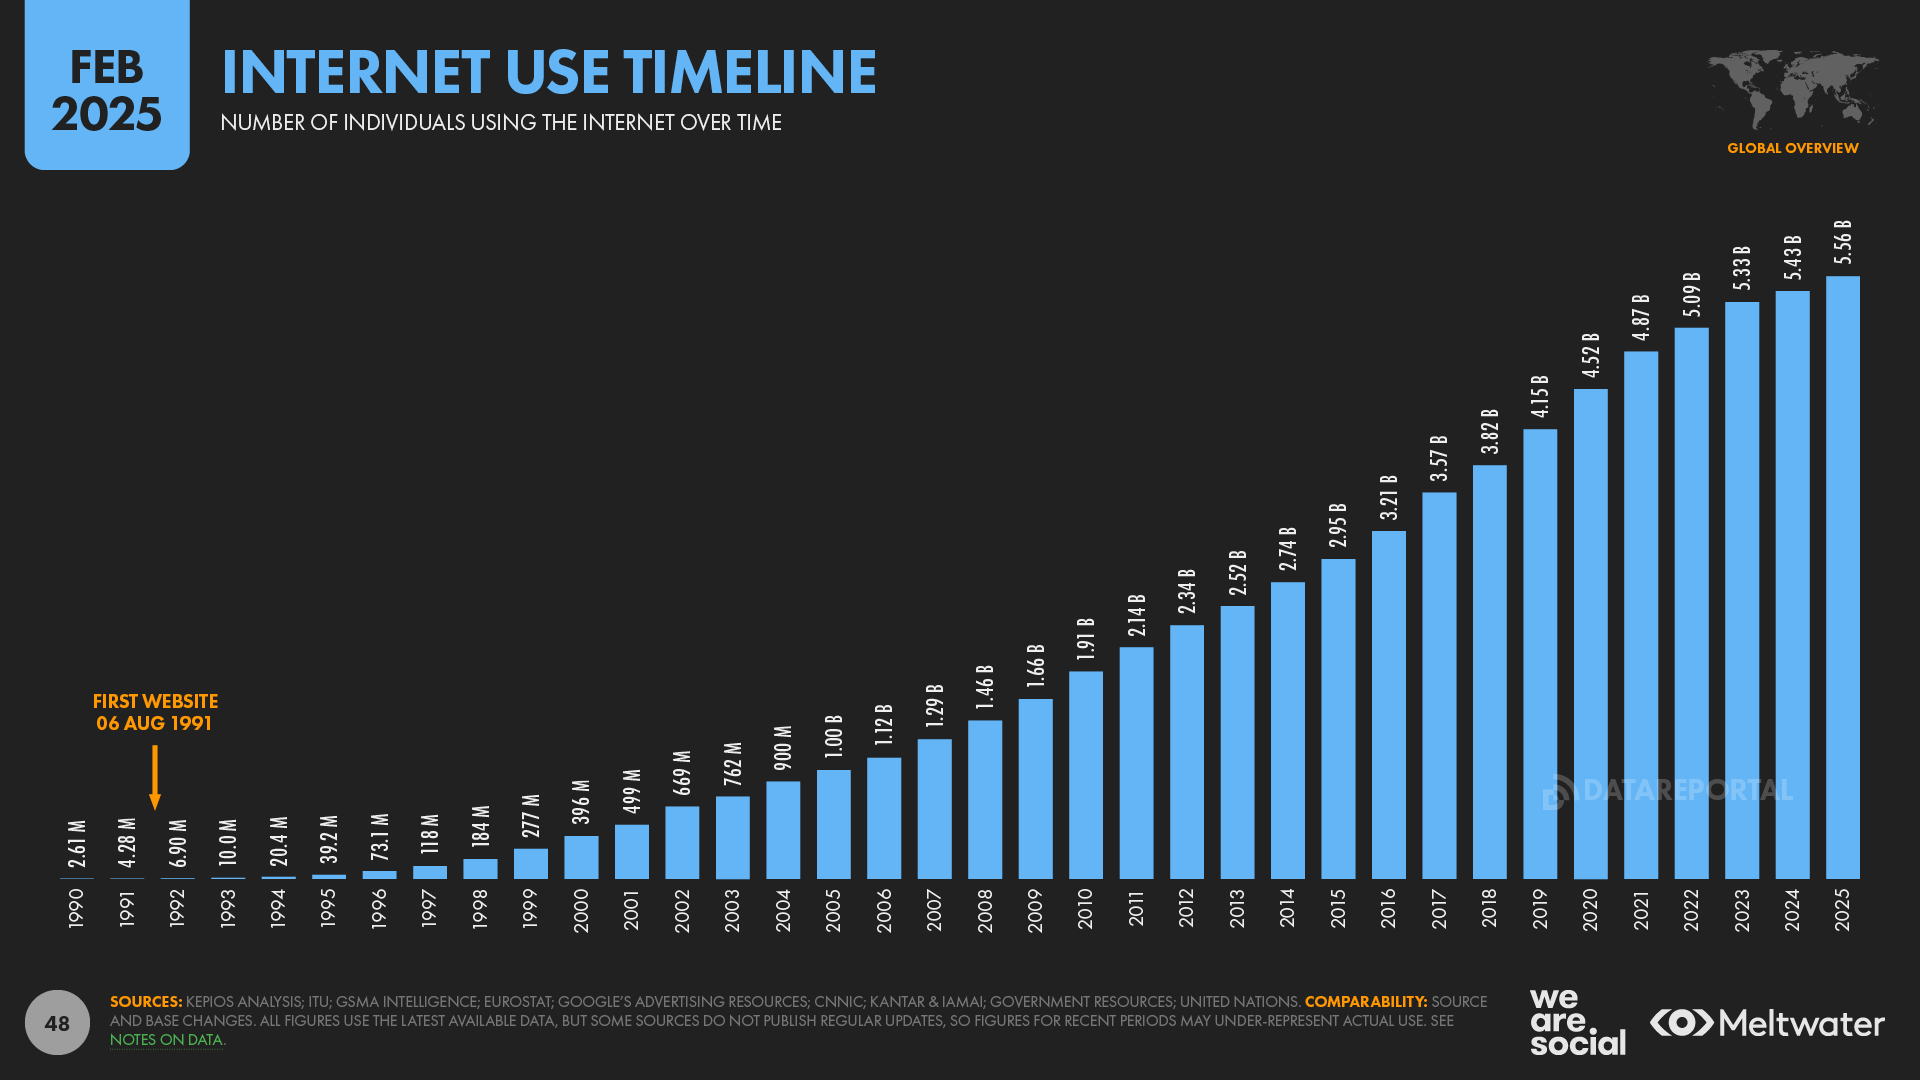
\includegraphics[width=0.8\pagewidth]{../network/internet_users.png}
\end{center}
\end{frame}

\begin{frame}{}
\begin{center}
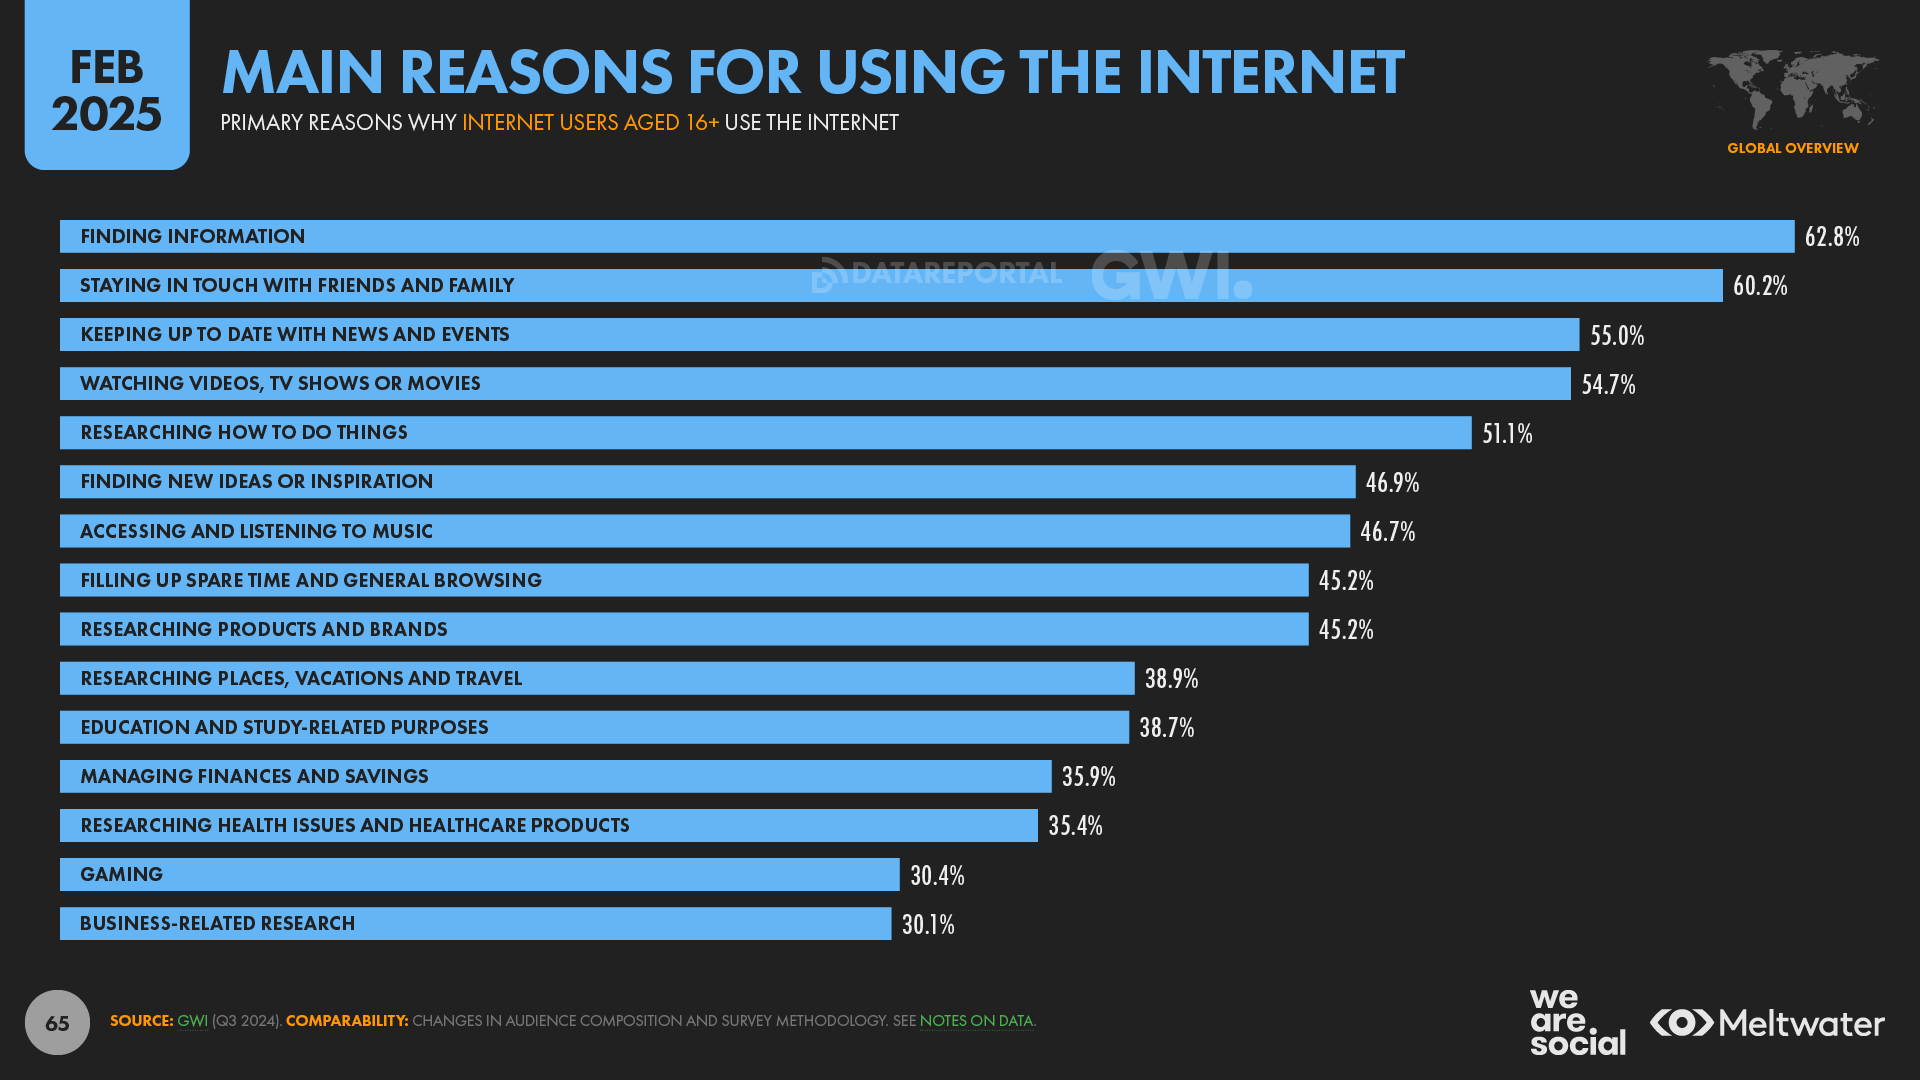
\includegraphics[width=0.8\pagewidth]{../network/internet_reasons.png}
\end{center}
\end{frame}

\begin{frame}{}
\begin{center}
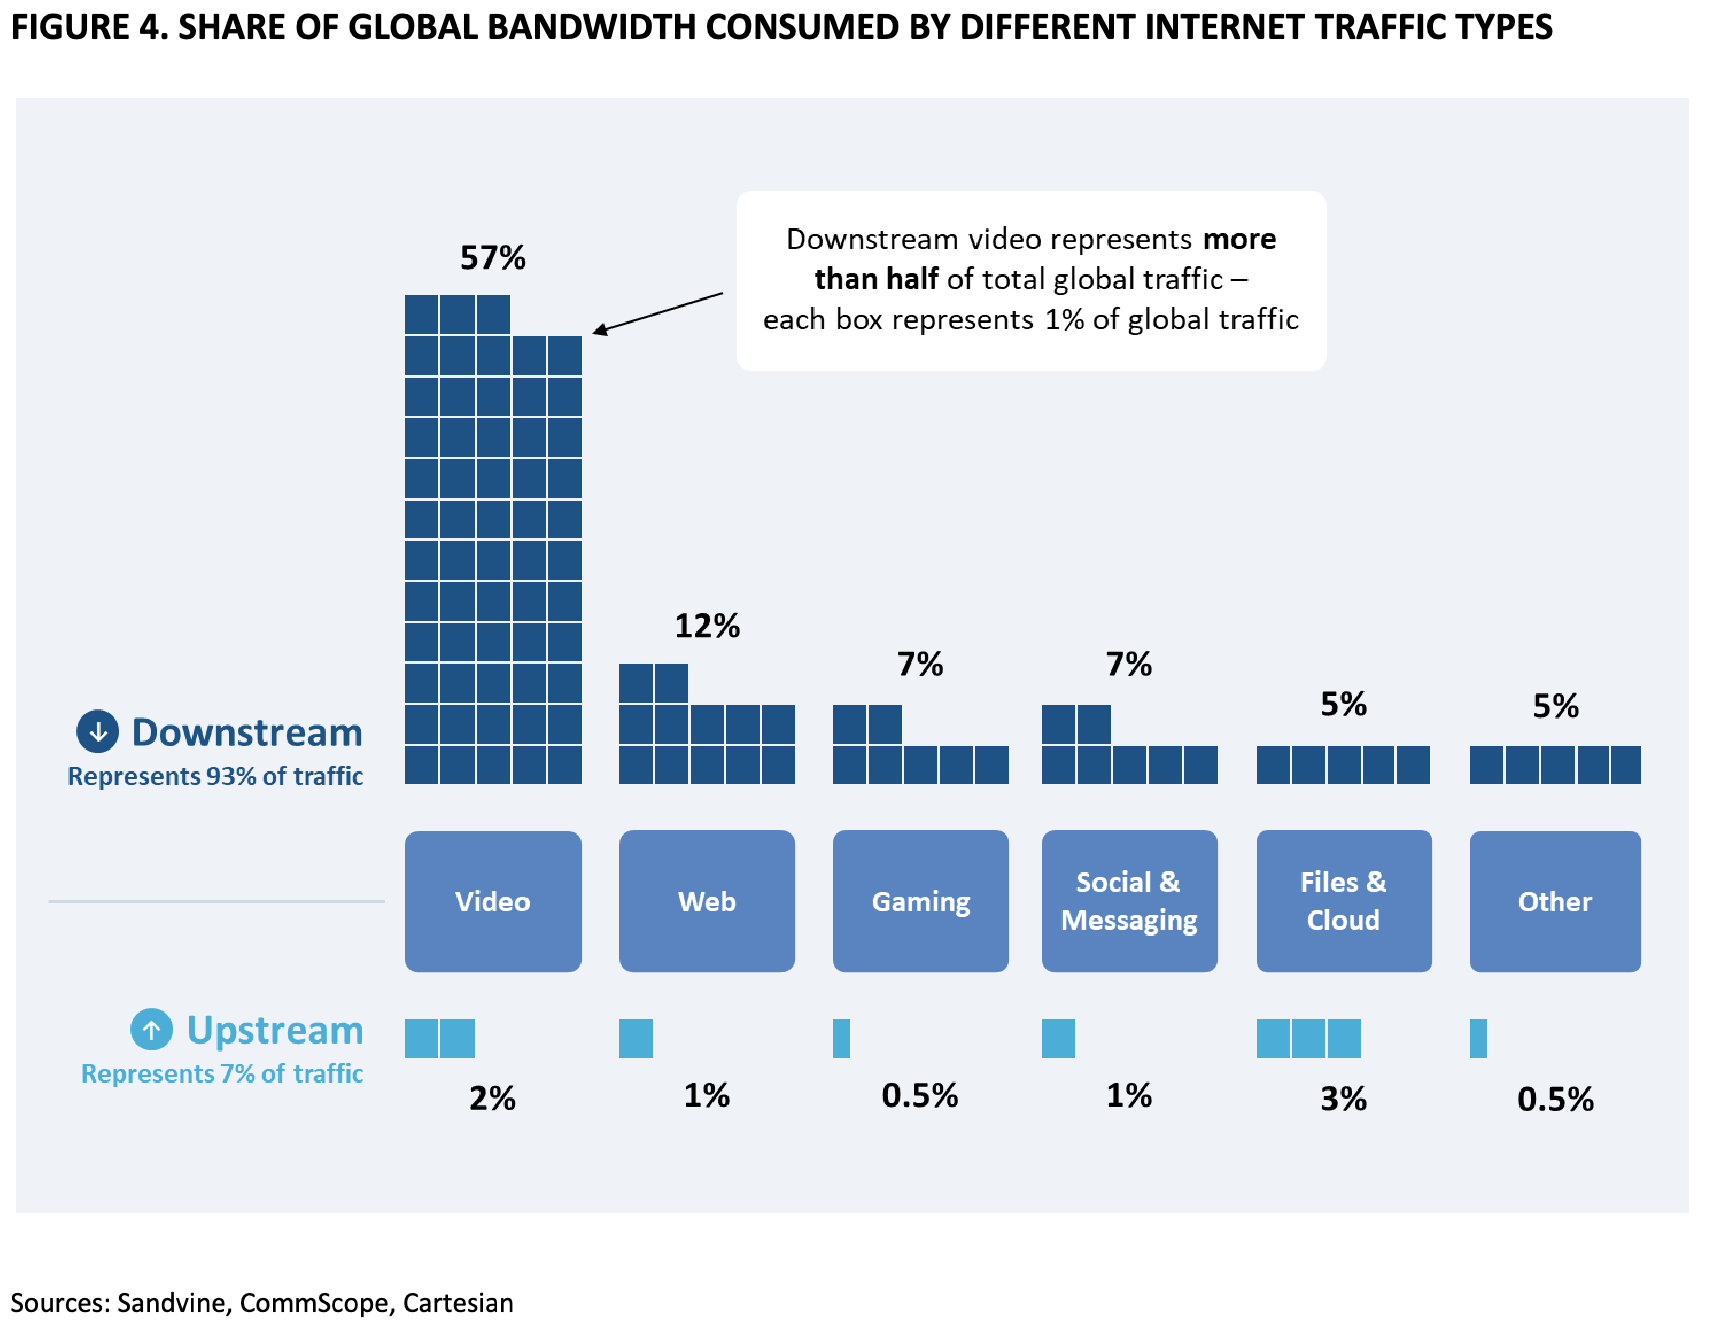
\includegraphics[width=0.8\pagewidth]{../network/internet_data.png}
\end{center}
\end{frame}

\section{ethernet / 802.11 / \ldots}
\begin{frame}{the link layer}
\begin{itemize}
\item Ethernet, Wi-Fi, Bluetooth, DOCSIS (cable modems), \ldots
\vspace{.5cm}
\item allows send/recv messages to machines on \myemph<2>{``same'' network segment}
    \begin{itemize}
    \item typically: wireless range+channel or connected to a single switch/router
    \item could be larger (if \textit{bridging} multiple network segments)
    \item could be smaller (switch/router uses ``virtual LANs'')
    \end{itemize}
\item typically: source+destination specified with MAC addresses
    \begin{itemize}
    \item MAC = media access control
    \item usually manufacturer assigned / hard-coded into device
    \item unique address per port/wifi transmitter/etc.
    \end{itemize}
\item can specify destination of ``anyone'' (called \textit{broadcast})
\item messages usually called ``frames''
\end{itemize}
\end{frame}

\begin{frame}{link layer jobs}
    \begin{itemize}
    \item divide raw bits into messages
    \item identify who message is for on shared radio/wire
    \item handle if two+ machines use radio/wire at same time
    \item drop/resend messages if corruption detected
        \begin{itemize}
        \item resending more common in radio schemes (wifi, etc.)
        \end{itemize}
    \end{itemize}
\end{frame}


\subsection{exercise: why resend?}
\begin{frame}{link layer reliablity?}
    \begin{itemize}
    \item Ethernet + Wifi have checksums
    \vspace{.5cm}
    \item Q1: Why doesn't this give us uncorrupted messages?
        \begin{itemize}
        \item Why do we still have checksums at the higher layers?
        \end{itemize}
    \item Q2: What's a benefit of doing this if we're also doing it in the higher layer?
    \end{itemize}
\end{frame}



\subsection{link layer quality-of-service}

\begin{frame}{link layer quality of service}
if frame gets\ldots \\
\small
\begin{tabular}{l|l|l}
event & on Ethernet & on WiFi \\\hline
collides with another & detected + may resend & resend\\
not received & lose silently & resent \\
header corrupted & usually discard silently & usually resend \\
data corrupted & usually discard silently & usually resend \\
too long & not allowed to send & not allowed to send \\
reordered (v. other messages)  & received out of order & received out of order \\
destination unknown & lose silently & usually resend?? \\
too much being sent & discard excess? & discard excess? \\
\end{tabular}
\end{frame}


\subsection{network layer quality-of-service}

\begin{frame}[fragile]{network layer quality of service}
if packet \ldots \\
\small
\begin{tabular}{l|p{12cm}}
event & on IPv4/v6 \\\hline
collides with another & out of scope --- handled by link layer \\
\myemph<2>{not received}\tikzmark{not recv} & lost silently \\
header corrupted & usually discarded silently \\
data corrupted & received corrupted \\
too long & dropped with notice or ``fragmented'' + recombined \\
reordered (v. other messages) & received out of order \\
destination unknown & usually dropped with notice \\
too much being sent & discard excess \\
\end{tabular}
\begin{tikzpicture}[overlay,remember picture]
\begin{visibleenv}<2>
\node[align=left,my callout=not recv,anchor=north west] at ([xshift=0cm,yshift=-3cm]pic cs:not recv) {
    includes dropped by link layer \\
    (e.g. if detected corrupted there)
};
\end{visibleenv}
\end{tikzpicture}
\end{frame}


\section{firewalls} % FIXME: complete
\begin{frame}{firewalls}
    \begin{itemize}
    \item don't want to expose network service to everyone?
    \item solutions:
        \begin{itemize}
        \item service picky about who it accepts connections from
        \item filters in OS on machine with services
        \item filters on router
        \end{itemize}
    \item later two called ``firewalls''
    \end{itemize}
\end{frame}

\begin{frame}{firewall rules examples?}
    \begin{itemize}
    \item ALLOW tcp port 443 (https) FROM everyone
    \item ALLOW tcp port 22 (ssh) FROM \myemph{my desktop's IP address}
    \item BLOCK tcp port 22 (ssh) FROM everyone else
    \item ALLOW from address X to address Y
    \item \ldots
    \end{itemize}
\end{frame}



\subsection{aside: TCP state machine}
\begin{frame}{TCP state machine}
\begin{itemize}
\item TIME\_WAIT, ESTABLISHED, \ldots?
\vspace{.5cm}
\item OS tracks ``state'' of TCP connection
    \begin{itemize}
    \item am I just starting the connection?
    \item is other end ready to get data?
    \item am I trying to close the connection?
    \item do I need to resend something?
    \end{itemize}
\item standardized set of state names
\end{itemize}
\end{frame}


\begin{frame}{TIME\_WAIT}
\begin{itemize}
\item remember delayed messages?
\vspace{.5cm}
\item problem for TCP ports
\item if I reuse port number, I can get message from old connection
\item solution: TIME\_WAIT to make sure connection really done
    \begin{itemize}
    \item done after sending last message in connection
    \end{itemize}
\end{itemize}
\end{frame}
 % FIXME: diagram
\subsection{DIG trace}

\begin{frame}[fragile]{querying the root}
\begin{Verbatim}[fontsize=\scriptsize]
$ dig @a.root-servers.net www.cs.virginia.edu
...
edu.			172800	IN	NS	b.edu-servers.net.
edu.			172800	IN	NS	f.edu-servers.net.
edu.			172800	IN	NS	i.edu-servers.net.
edu.			172800	IN	NS	a.edu-servers.net.
...
b.edu-servers.net.	172800	IN	A	192.33.14.30
b.edu-servers.net.	172800	IN	AAAA	2001:503:231d::2:30
f.edu-servers.net.	172800	IN	A	192.35.51.30
f.edu-servers.net.	172800	IN	AAAA	2001:503:d414::30
...
\end{Verbatim}
\end{frame}

\begin{frame}[fragile]{querying the edu}
\begin{Verbatim}[fontsize=\scriptsize]
$ dig @b.edu-servers.net www.cs.virginia.edu
...
;; AUTHORITY SECTION:
virginia.edu.		172800	IN	NS	nom.virginia.edu.
virginia.edu.		172800	IN	NS	uvaarpa.virginia.edu.
virginia.edu.		172800	IN	NS	eip-01-aws.net.virginia.edu.

;; ADDITIONAL SECTION:
nom.virginia.edu.	172800	IN	A	128.143.107.101
uvaarpa.virginia.edu.	172800	IN	A	128.143.107.117
eip-01-aws.net.virginia.edu. 172800 IN	A	44.234.207.10
\end{Verbatim}
\end{frame}
\begin{frame}[fragile]{querying virginia.edu}
\begin{Verbatim}[fontsize=\scriptsize]
$ dig @nom.virginia.edu www.cs.virginia.edu
...
;; AUTHORITY SECTION:
cs.virginia.edu.	3600	IN	NS	coresrv01.cs.virginia.edu.

;; ADDITIONAL SECTION:
coresrv01.cs.virginia.edu. 3600	IN	A	128.143.67.11
\end{Verbatim}
\end{frame}

\begin{frame}[fragile]{querying cs.virginia.edu}
\begin{Verbatim}[fontsize=\scriptsize]
$ dig @coresrv01.cs.virginia.edu
...
;; ANSWER SECTION:
www.cs.Virginia.EDU.	172800	IN	A	128.143.67.11

;; AUTHORITY SECTION:
cs.Virginia.EDU.	172800	IN	NS	coresrv01.cs.Virginia.EDU.
...
\end{Verbatim}
\end{frame}

\begin{frame}[fragile]{querying typical ISP's resolver}
\begin{Verbatim}[fontsize=\scriptsize]
$ dig www.cs.virginia.edu
...
;; ANSWER SECTION:
www.cs.Virginia.EDU.	  7183	IN	A	128.143.67.11
..
\end{Verbatim}
\begin{itemize}
\item cached response
\item valid for 7183  more seconds
\item after that everyone needs to check again
\end{itemize}
\end{frame}


\subsection{UDP sockets}
\begin{frame}[fragile]{UDP sockets on IPv4}
\begin{lstlisting}[language=C++,style=smaller]
int fd = socket(AF_INET, SOCK_DGRAM, 0);
struct sockaddr_in my_addr= ...;
bind(fd, &my_addr, sizeof(my_addr))
...
struct sockaddr_in to_addr = ...;
sendto(fd, data, data_size, 0 /* flags */,
    &to_addr, sizeof(to_addr));
struct sockaddr_in from_addr = ...;
recvfrom(fd, &buffer[0], buffer_size, 0,
    &from_addr, sizeof(from_addr));
...
/* or connect() to set default sendto address
\end{lstlisting}
\end{frame}


\subsection{ARP / IPv6 ND routing}

\begin{frame}{what about non-local machines?}
    \begin{itemize}
    \item when configuring network specify:
    \vspace{.5cm}
    \item range of addresses to expect on local network 
        \begin{itemize}
        \item 128.148.67.0-128.148.67.255 on my desktop
        \item ``netmask''
        \end{itemize}
    \item \textit{gateway} machine to send to for things outside my local network
        \begin{itemize}
        \item 128.143.67.1 on my desktop
        \item my desktop looks up the corresponding MAC address
        \end{itemize}
    \end{itemize}
\end{frame}

\begin{frame}[fragile]{routes on my desktop}
\begin{Verbatim}[fontsize=\fontsize{9}{10}\selectfont]
$ /sbin/route -n
Kernel IP routing table
Destination     Gateway         Genmask         Flags Metric Ref    Use Iface
0.0.0.0         128.143.67.1    0.0.0.0         UG    100    0        0 enp0s31f6
128.143.67.0    0.0.0.0         255.255.255.0   U     100    0        0 enp0s31f6
169.254.0.0     0.0.0.0         255.255.0.0     U     1000   0        0 enp0s31f6
\end{Verbatim}
\begin{itemize}
\item network configuration says:
\vspace{.5cm}
\item (line 2) to get to 128.143.67.0--128.143.67.255, send directly on local network
    \begin{itemize}
    \item ``genmask'' is mask (for bitwise operations) to specify how big range is
    \end{itemize}
\item (line 3) to get to 169.254.0.0--169.254.255.255, send directly on local network
\item (line 1) to get anywhere else, use ``gateway'' 128.143.67.1
\end{itemize}
\end{frame}


\subsection{ARP / IPv6 ND}
\againframe<3>{nameAndAddr}
\begin{frame}{two types of addresses?}
    \begin{itemize}
    \item MAC addreses: on link layer
    \item IP addresses: on network layer
    \vspace{.5cm}
    \item how do we know which MAC address to use?
    \end{itemize}
\end{frame}

\begin{frame}[fragile]{a table on my desktop}
my desktop: \\
\begin{Verbatim}[fontsize=\fontsize{9}{10}\selectfont]
$ arp -an
? (128.143.67.140) at 3c:e1:a1:18:bd:5f [ether] on enp0s31f6
? (128.143.67.236) at <incomplete> on enp0s31f6
? (128.143.67.11) at 30:e1:71:5f:39:10 [ether] on enp0s31f6
? (128.143.67.92) at <incomplete> on enp0s31f6
? (128.143.67.5) at d4:be:d9:b0:99:d1 [ether] on enp0s31f6
\end{Verbatim}
\ldots
\end{frame}

\begin{frame}{how is that table made?}
    \begin{itemize}
    \item ask machines on local network (same switch)
    \item ``Who has 128.148.67.140''
    \item the correct one replies
    \end{itemize}
\end{frame}

\begin{frame}{what about non-local machines?}
    \begin{itemize}
    \item when configuring network specify:
    \vspace{.5cm}
    \item range of addresses to expect on local network 
        \begin{itemize}
        \item 128.148.67.0-128.148.67.255 on my desktop
        \item ``netmask''
        \end{itemize}
    \item \textit{gateway} machine to send to for things outside my local network
        \begin{itemize}
        \item 128.143.67.1 on my desktop
        \item my desktop looks up the corresponding MAC address
        \end{itemize}
    \end{itemize}
\end{frame}

\begin{frame}[fragile]{routes on my desktop}
\begin{Verbatim}[fontsize=\fontsize{9}{10}\selectfont]
$ /sbin/route -n
Kernel IP routing table
Destination     Gateway         Genmask         Flags Metric Ref    Use Iface
0.0.0.0         128.143.67.1    0.0.0.0         UG    100    0        0 enp0s31f6
128.143.67.0    0.0.0.0         255.255.255.0   U     100    0        0 enp0s31f6
169.254.0.0     0.0.0.0         255.255.0.0     U     1000   0        0 enp0s31f6
\end{Verbatim}
\begin{itemize}
\item network configuration says:
\vspace{.5cm}
\item (line 2) to get to 128.143.67.0--128.143.67.255, send directly on local network
    \begin{itemize}
    \item ``genmask'' is mask (for bitwise operations) to specify how big range is
    \end{itemize}
\item (line 3) to get to 169.254.0.0--169.254.255.255, send directly on local network
\item (line 1) to get anywhere else, use ``gateway'' 128.143.67.1
\end{itemize}
\end{frame}


% FIXME: HTTP request/response?
\section{and HTTP? (exercise)}
\begin{frame}[fragile]{URLs and HTTP (1)}
\begin{itemize}
    \item \texttt{http://www.foo.com:80/foo/bar?quux\myemph<2>{\#q1}}
    \item lookup IP address of www.foo.com
    \item connect via TCP to port 80:
\end{itemize}
\providecommand{\emphThree}[1]{\myemph<3>{#1}}
\begin{Verbatim}[commandchars=X()]
GET /foo/bar?quux HTTP/1.1
Host: XemphThree(www.foo.com:80)
\end{Verbatim}
\begin{itemize}
    \item<3-> exercise: why include the Host there?
\end{itemize}
\end{frame}



% FIXME: DNS dig example
\subsection{DNS: dig +trace}

\begin{frame}[fragile]{querying the root}
\begin{Verbatim}[fontsize=\scriptsize]
$ dig @a.root-servers.net www.cs.virginia.edu
...
edu.			172800	IN	NS	b.edu-servers.net.
edu.			172800	IN	NS	f.edu-servers.net.
edu.			172800	IN	NS	i.edu-servers.net.
edu.			172800	IN	NS	a.edu-servers.net.
...
b.edu-servers.net.	172800	IN	A	192.33.14.30
b.edu-servers.net.	172800	IN	AAAA	2001:503:231d::2:30
f.edu-servers.net.	172800	IN	A	192.35.51.30
f.edu-servers.net.	172800	IN	AAAA	2001:503:d414::30
...
\end{Verbatim}
\end{frame}

\begin{frame}[fragile]{querying the edu}
\begin{Verbatim}[fontsize=\scriptsize]
$ dig @b.edu-servers.net www.cs.virginia.edu
...
;; AUTHORITY SECTION:
virginia.edu.		172800	IN	NS	nom.virginia.edu.
virginia.edu.		172800	IN	NS	uvaarpa.virginia.edu.
virginia.edu.		172800	IN	NS	eip-01-aws.net.virginia.edu.

;; ADDITIONAL SECTION:
nom.virginia.edu.	172800	IN	A	128.143.107.101
uvaarpa.virginia.edu.	172800	IN	A	128.143.107.117
eip-01-aws.net.virginia.edu. 172800 IN	A	44.234.207.10
\end{Verbatim}
\end{frame}
\begin{frame}[fragile]{querying virginia.edu}
\begin{Verbatim}[fontsize=\scriptsize]
$ dig @nom.virginia.edu www.cs.virginia.edu
...
;; AUTHORITY SECTION:
cs.virginia.edu.	3600	IN	NS	coresrv01.cs.virginia.edu.

;; ADDITIONAL SECTION:
coresrv01.cs.virginia.edu. 3600	IN	A	128.143.67.11
\end{Verbatim}
\end{frame}

\begin{frame}[fragile]{querying cs.virginia.edu}
\begin{Verbatim}[fontsize=\scriptsize]
$ dig @coresrv01.cs.virginia.edu
...
;; ANSWER SECTION:
www.cs.Virginia.EDU.	172800	IN	A	128.143.67.11

;; AUTHORITY SECTION:
cs.Virginia.EDU.	172800	IN	NS	coresrv01.cs.Virginia.EDU.
...
\end{Verbatim}
\end{frame}

\begin{frame}[fragile]{querying typical ISP's resolver}
\begin{Verbatim}[fontsize=\scriptsize]
$ dig www.cs.virginia.edu
...
;; ANSWER SECTION:
www.cs.Virginia.EDU.	  7183	IN	A	128.143.67.11
..
\end{Verbatim}
\begin{itemize}
\item cached response
\item valid for 7183  more seconds
\item after that everyone needs to check again
\end{itemize}
\end{frame}


\section{spoofing?}
\begin{frame}{spoofing}
    \begin{itemize}
    \item if I only allow connections from my desktop's IP addresses, \\
        how would you attack this?
    \vspace{.5cm}
    \item hint: how do we know what address messages come from?
    \end{itemize}
\end{frame}



\subsection{example: echo client/server}
\subsubsection{server setup}
\begin{frame}[fragile,label=connSetupServer]{connection setup: server, manual}
\begin{lstlisting}[
    language=C++,style=smaller,
    moredelim={**[is][\btHL<2|handout:2>]{@2}{2@}},
    moredelim={**[is][\btHL<3|handout:3>]{@3}{3@}},
    moredelim={**[is][\btHL<4|handout:4>]{@4}{4@}},
    moredelim={**[is][\btHL<5|handout:5>]{@5}{5@}},
    moredelim={**[is][\btHL<6|handout:6>]{@6}{6@}},
]
int server_socket_fd = socket(AF_INET, SOCK_STREAM, IPPROTO_TCP);
struct sockaddr_in addr;
addr.sin_family = AF_INET;
addr.sin_addr.s_addr = @2INADDR_ANY2@; /* "any address I can use" */
    @3/* or: addr.s_addr.in_addr = INADDR_LOOPBACK (127.0.0.1) */3@
    /* or: addr.s_addr.in_addr = htonl(...); */
addr.sin_port = @4htons(9999)4@; /* port number 9999 */

if (bind(server_socket_fd, &addr, sizeof(addr)) < 0) {
    /* handle error */
}
listen(server_socket_fd, @4MAX_NUM_WAITING4@);
...
int socket_fd = accept(server_socket_fd, NULL);
\end{lstlisting}
\begin{tikzpicture}[overlay,remember picture]
\tikzset{
    box/.style={draw=red, ultra thick,fill=white,at={([yshift=-2cm]current page.north)},anchor=north,align=left},
    box low/.style={draw=red, ultra thick,fill=white,at={([yshift=-6cm]current page.north)},anchor=north,align=left},
}
\begin{visibleenv}<2>
\node[box low] {
    INADDR\_ANY: accept connections for any address I can! \\
    alternative: specify specific address
};
\end{visibleenv}
\begin{visibleenv}<3>
\node[box low] {
    bind to 127.0.0.1? only accept connections \myemph{from same machine} \\
    what we recommend for FTP server assignment
};
\end{visibleenv}
\begin{visibleenv}<4>
\node[box low] {
    choose the number of unaccepted connections
};
\end{visibleenv}
\end{tikzpicture}
\end{frame}

\subsubsection{client setup}
\begin{frame}[fragile,label=connSetupClientManual]{connection setup: client --- manual addresses}
\begin{lstlisting}[
    language=C++,style=smaller,
    moredelim={**[is][\btHL<1|handout:1>]{@1}{1@}},
    moredelim={**[is][\btHL<2|handout:2>]{@2}{2@}},
    moredelim={**[is][\btHL<3|handout:3>]{@3}{3@}},
    moredelim={**[is][\btHL<4|handout:4>]{@4}{4@}},
    moredelim={**[is][\btHL<5|handout:5>]{@5}{5@}},
    moredelim={**[is][\btHL<6|handout:6>]{@6}{6@}},
]
int sock_fd;

server = /* code on later slide */;
sock_fd = @1socket1@(
    @2AF_INET2@, /* IPv4 */
    @2SOCK_STREAM2@, /* byte-oriented */
    @2IPPROTO_TCP2@
);
if (sock_fd < 0) { /* handle error */ }

@4struct sockaddr_in addr4@;
addr.sin_family = AF_INET;
addr.sin_addr.s_addr = @3htonl3@(2156872459); /* 128.143.67.11 */
addr.sin_port = @3htons3@(80); /* port 80 */
if (@1connect1@(sock_fd, (struct sockaddr*) &addr, sizeof(addr)) {
    /* handle error */
}
DoClientStuff(sock_fd); /* read and write from sock_fd */
close(sock_fd);
\end{lstlisting}
\begin{tikzpicture}[overlay,remember picture]
\tikzset{
    box/.style={draw=red, ultra thick,fill=white,at={([yshift=-2cm]current page.north)},anchor=north,align=left},
    box low/.style={draw=red, ultra thick,fill=white,at={([yshift=-5cm]current page.north)},anchor=north,align=left},
}
\begin{visibleenv}<2>
\node[box low] {
    specify IPv4 instead of IPv6 or local-only sockets \\
    specify TCP (byte-oriented) instead of UDP (`datagram' oriented)
};
\end{visibleenv}
\begin{visibleenv}<3>
\node[box] {
    htonl/s = host-to-network long/short \\
    network byte order = big endian
};
\end{visibleenv}
\begin{visibleenv}<4>
\node[box] {
    struct representing IPv4 address + port number \\
    declared in \lstinline|<netinet/in.h>| \\
    see \texttt{man 7 ip} on Linux for docs
};
\end{visibleenv}
\end{tikzpicture}
\end{frame}


\subsubsection{read/write code}

\begin{frame}[fragile,label=echoClient]{echo client/server}
\begin{lstlisting}[
    language=C++,
    basicstyle=\sourcecodepro\EmptyMapping\fontsize{10}{11}\selectfont,
    keywordstyle=\sourcecodepro\EmptyMapping\fontsize{10}{11}\selectfont,
    moredelim={**[is][\btHL<1|handout:1>]{@1}{1@}},
    moredelim={**[is][\btHL<2|handout:2>]{@2}{2@}},
    moredelim={**[is][\btHL<3|handout:3>]{@3}{3@}},
    moredelim={**[is][\btHL<4|handout:4>]{@4}{4@}},
    moredelim={**[is][\btHL<5|handout:5>]{@5}{5@}},
    moredelim={**[is][\btHL<6|handout:6>]{@6}{6@}},
]
void client_for_connection(int socket_fd) {
    int n; char send_buf[MAX_SIZE]; char recv_buf[MAX_SIZE];
    while (prompt_for_input(send_buf, MAX_SIZE)) {
        n = @2write(socket_fd, send_buf, strlen(send_buf))2@;
        if (n != strlen(send_buf)) {...error?...}
        n = @3read(socket_fd, recv_buf, MAX_SIZE)3@;
        if (n <= 0) return; // error or EOF 
        write(STDOUT_FILENO, recv_buf, n);
    }
}
\end{lstlisting}
\hrule
\begin{lstlisting}[
    language=C++,style=smaller,
    moredelim={**[is][\btHL<1|handout:1>]{@1}{1@}},
    moredelim={**[is][\btHL<2|handout:2>]{@2}{2@}},
    moredelim={**[is][\btHL<3|handout:3>]{@3}{3@}},
    moredelim={**[is][\btHL<4|handout:4>]{@4}{4@}},
    moredelim={**[is][\btHL<5|handout:5>]{@5}{5@}},
    moredelim={**[is][\btHL<6|handout:6>]{@6}{6@}},
]
void server_for_connection(int socket_fd) {
    int read_count, write_count; char request_buf[MAX_SIZE];
    while (1) {
        read_count = @2read(socket_fd, request_buf, MAX_SIZE)2@;
        if (read_count <= 0) return; // error or EOF 
        write_count = @3write(socket_fd, request_buf, read_count)3@;
        if (read_count != write_count) {...error?...}
    }
}
\end{lstlisting}
\end{frame}



\subsection{more normal connection setup}
\begin{frame}[fragile,label=connSetupServerLookup]{connection setup: server, address setup}
\begin{lstlisting}[
    language=C++,style=smaller,
    moredelim={**[is][\btHL<2|handout:2>]{@2}{2@}},
    moredelim={**[is][\btHL<3|handout:3>]{@3}{3@}},
    moredelim={**[is][\btHL<4|handout:4>]{@4}{4@}},
    moredelim={**[is][\btHL<5|handout:5>]{@5}{5@}},
    moredelim={**[is][\btHL<6|handout:6>]{@6}{6@}},
]
/* example (hostname, portname) = ("127.0.0.1", "443") */
const char *@2hostname2@; const char *@3portname3@;
...
struct addrinfo *server;
struct addrinfo hints;
int rv;

memset(&hints, 0, sizeof(hints));
hints.ai_family = AF_INET; /* for IPv4 */
/* or: */ hints.ai_family = AF_INET6; /* for IPv6 */
/* or: */ hints.ai_family = AF_UNSPEC; /* I don't care */
@4hints.ai_flags = AI_PASSIVE4@;

rv = getaddrinfo(hostname, portname, &hints, &server);
if (rv != 0) { /* handle error */ }
\end{lstlisting}
\begin{tikzpicture}[overlay,remember picture]
\tikzset{
    box/.style={draw=red, ultra thick,fill=white,at={([yshift=-2cm]current page.north)},anchor=north,align=left},
    box low/.style={draw=red, ultra thick,fill=white,at={([yshift=-6cm]current page.north)},anchor=north,align=left},
}
\begin{visibleenv}<2>
\node[box low] {
    \texttt{hostname} could also be NULL \\
    means ``use all possible addresses'' \\
    only makes sense for servers
};
\end{visibleenv}
\begin{visibleenv}<3>
\node[box low] {
    \texttt{portname} could also be NULL \\
    means ``choose a port number for me'' \\
    only makes sense for servers
};
\end{visibleenv}
\begin{visibleenv}<4>
\node[box] {
    AI\_PASSIVE: ``I'm going to use bind''
};
\end{visibleenv}
\end{tikzpicture}
\end{frame}


\begin{frame}[fragile,label=connSetupServerAddrinfo]{connection setup: server, addrinfo}
\begin{lstlisting}[
    language=C++,style=smaller,
    moredelim={**[is][\btHL<2|handout:2>]{@2}{2@}},
    moredelim={**[is][\btHL<3|handout:3>]{@3}{3@}},
    moredelim={**[is][\btHL<4|handout:4>]{@4}{4@}},
    moredelim={**[is][\btHL<5|handout:5>]{@5}{5@}},
    moredelim={**[is][\btHL<6|handout:6>]{@6}{6@}},
]
struct addrinfo *server;
... getaddrinfo(...) ...

int server_socket_fd = socket(
    server->ai_family,
    server->ai_sockttype,
    server->ai_protocol
);

if (bind(server_socket_fd, ai->ai_addr, ai->ai_addr_len)) < 0) {
    /* handle error */
}
listen(server_socket_fd, MAX_NUM_WAITING);
...
int socket_fd = accept(server_socket_fd, NULL);
\end{lstlisting}
\end{frame}


\begin{frame}[fragile,label=connSetupClientAddrInfo]{connection setup: client, using addrinfo}
\begin{lstlisting}[
    language=C++,style=smaller,
    moredelim={**[is][\btHL<2|handout:2>]{@2}{2@}},
    moredelim={**[is][\btHL<3|handout:3>]{@3}{3@}},
    moredelim={**[is][\btHL<4|handout:4>]{@4}{4@}},
    moredelim={**[is][\btHL<5|handout:5>]{@5}{5@}},
    moredelim={**[is][\btHL<6|handout:6>]{@6}{6@}},
]
int sock_fd; 
@2struct addrinfo2@ *server = /* code on next slide */;

sock_fd = socket(
    @3server->ai_family3@,  
     // ai_family = AF_INET (IPv4) or AF_INET6 (IPv6) or ...
    @3server->ai_socktype3@,
     // ai_socktype = SOCK_STREAM (bytes) or ...
    @3server->ai_prototcol3@
     // ai_protocol = IPPROTO_TCP or ...
);
if (sock_fd < 0) { /* handle error */ }
if (connect(sock_fd, server->@4ai_addr4@, server->@4ai_addrlen4@) < 0) {
    /* handle error */
}
@5freeaddrinfo(server);5@
DoClientStuff(sock_fd); /* read and write from sock_fd */
close(sock_fd);
\end{lstlisting}
\begin{tikzpicture}[overlay,remember picture]
\tikzset{
    box/.style={draw=red, ultra thick,fill=white,at={([yshift=-2cm]current page.north)},anchor=north,align=left},
    box low/.style={draw=red, ultra thick,fill=white,at={([yshift=-5cm]current page.north)},anchor=north,align=left},
}
\begin{visibleenv}<2>
\node[box low] {
    addrinfo contains all information needed to setup socket \\
    set by \texttt{getaddrinfo} function (next slide) \\
    handles IPv4 and IPv6 \\
    handles DNS names, service names
};
\end{visibleenv}
\begin{visibleenv}<4>
\node[box] {
    ai\_addr points to struct representing address \\
    type of struct depends whether IPv6 or IPv4
};
\end{visibleenv}
\begin{visibleenv}<5>
\node[box] {
    since addrinfo contains pointers to dynamically allocated memory, \\
    call this function to free everything
};
\end{visibleenv}
\end{tikzpicture}
\end{frame}

\begin{frame}[fragile,label=serverLookupClient]{connection setup: lookup address}
\begin{lstlisting}[
    language=C++,style=smaller,
    moredelim={**[is][\btHL<2|handout:2>]{@2}{2@}},
    moredelim={**[is][\btHL<3|handout:3>]{@3}{3@}},
    moredelim={**[is][\btHL<4|handout:4>]{@4}{4@}},
    moredelim={**[is][\btHL<5|handout:5>]{@5}{5@}},
    moredelim={**[is][\btHL<6|handout:6>]{@6}{6@}},
]
/* example hostname, portname = "www.cs.virginia.edu", "443" */
const char *hostname; const char *portname;
...
struct addrinfo *server;
struct addrinfo hints;
int rv;
memset(&hints, 0, sizeof(hints));
@3hints.ai_family = AF_UNSPEC3@; /* for IPv4 OR IPv6 */
// hints.ai_family = AF_INET4; /* for IPv4 only */

hints.ai_socktype = SOCK_STREAM; /* byte-oriented --- TCP */
rv = getaddrinfo(hostname, portname, &hints, @2&server2@);
if (rv != 0) { /* handle error */ }

/* eventually freeaddrinfo(result) */
\end{lstlisting}
\begin{tikzpicture}[overlay,remember picture]
\tikzset{
    box/.style={draw=red, ultra thick,fill=white,at={([yshift=-2cm]current page.north)},anchor=north,align=left},
    box low/.style={draw=red, ultra thick,fill=white,at={([yshift=-5cm]current page.north)},anchor=north,align=left},
}
\begin{visibleenv}<2>
\node[box low] {
    NB: pass pointer \textit{to pointer} to addrinfo to fill in
};
\end{visibleenv}
\begin{visibleenv}<3>
\node[box] {
    AF\_UNSPEC: choose between IPv4 and IPv6 for me \\
    AF\_INET, AF\_INET6: choose IPv4 or IPV6 respectively
};
\end{visibleenv}
\end{tikzpicture}
\end{frame}


\subsection{other connection setup options}
\begin{frame}[fragile,label=serverLookupClientMulti]{connection setup: multiple server addresses}
\begin{lstlisting}[
    language=C++,style=smaller,
    moredelim={**[is][\btHL<2|handout:2>]{@2}{2@}},
    moredelim={**[is][\btHL<3|handout:3>]{@3}{3@}},
    moredelim={**[is][\btHL<4|handout:4>]{@4}{4@}},
    moredelim={**[is][\btHL<5|handout:5>]{@5}{5@}},
    moredelim={**[is][\btHL<6|handout:6>]{@6}{6@}},
]
struct addrinfo *server;
...
rv = getaddrinfo(hostname, portname, &hints, &server);
if (rv != 0) { /* handle error */ }

for (struct addrinfo *current = server; current != NULL;
      @2current = current->ai_next2@) {
    sock_fd = socket(current->ai_family, current->ai_socktype, current->ai_protocol);
    if (sock_fd < 0) continue;
    if (connect(sock_fd, current->ai_addr, current->ai_addrlen) == 0) {
        break;
    }
    close(sock_fd); // connect failed
}
freeaddrinfo(server);
DoClientStuff(sock_fd);
close(sock_fd);
\end{lstlisting}
\begin{tikzpicture}[overlay,remember picture]
\tikzset{
    box/.style={draw=red, ultra thick,fill=white,at={([yshift=-2cm]current page.north)},anchor=north,align=left},
    box low/.style={draw=red, ultra thick,fill=white,at={([yshift=-6.5cm]current page.north)},anchor=north,align=left},
}
\begin{visibleenv}<2>
\node[box low] {
    addrinfo is a linked list \\
    name can correspond to multiple addresses \\
    example: redundant copies of web server \\
    example: an IPv4 address and IPv6 address \\
    example: wired + wireless connection on one machine
};
\end{visibleenv}
\end{tikzpicture}
\end{frame}

\begin{frame}[fragile,label=serverLookupClientOld]{connection setup: old lookup function}
\begin{lstlisting}[language=C++,style=smaller]
/* example hostname, portnum= "www.cs.virginia.edu", 443*/
const char *hostname; int portnum;
...
struct hostent *server_ip;
server_ip = gethostbyname(hostname);

if (server_ip == NULL) { /* handle error */ }

struct sockaddr_in addr;
addr.s_addr = *(struct in_addr*) server_ip->h_addr_list[0];
addr.sin_port = htons(portnum);
sock_fd = socket(AF_INET, SOCK_STREAM, IPPROTO_TCP);
connect(sock_fd, &addr, sizeof(addr));
...
\end{lstlisting}
\end{frame}

\begin{frame}{aside: on server port numbers}
    \begin{itemize}
    \item Unix convention: must be \texttt{root} to use ports 0--1023
        \begin{itemize}
        \item root = superuser = `adminstrator user' = what sudo does
        \end{itemize}
    \item so, for testing: probably ports $>$ 1023
    \end{itemize}
\end{frame}



